% Needle thesis — generic report layout.
% Swap this preamble for the university template later; keep the \input lines.
% Chapters are generated: edit the Markdown in ../chapters, then run build.py.
\documentclass[12pt,a4paper,oneside]{report}

\usepackage{iftex}
\ifPDFTeX
  \usepackage[T1]{fontenc}
  \usepackage[utf8]{inputenc}
  \usepackage{lmodern}
\else
  \usepackage{fontspec}
\fi
\usepackage[margin=2.5cm]{geometry}
\usepackage{setspace}
\onehalfspacing
\usepackage{amsmath,amssymb}
\usepackage{graphicx}
\usepackage{longtable,booktabs,array,calc}
\usepackage{caption}
\newcounter{none} % pandoc's \LTcaptype{none} steps this instead of the table counter
\usepackage{fvextra} % wrap long lines in code blocks
\fvset{breaklines=true,breakanywhere=true,fontsize=\small}
\usepackage{xurl} % allow breaks inside long paths and URLs
\usepackage{xcolor}
\usepackage{upquote}
\usepackage[hidelinks]{hyperref}

% Macros that pandoc output expects.
\providecommand{\tightlist}{\setlength{\itemsep}{0pt}\setlength{\parskip}{0pt}}
\makeatletter
\newsavebox\pandoc@box
\newcommand*\pandocbounded[1]{%
  \sbox\pandoc@box{#1}%
  \Gscale@div\@tempa{\textheight}{\dimexpr\ht\pandoc@box+\dp\pandoc@box\relax}%
  \Gscale@div\@tempb{\linewidth}{\wd\pandoc@box}%
  \ifdim\@tempb\p@<\@tempa\p@\let\@tempa\@tempb\fi
  \ifdim\@tempa\p@<\p@\scalebox{\@tempa}{\usebox\pandoc@box}%
  \else\usebox{\pandoc@box}%
  \fi}
\makeatother
\setlength{\emergencystretch}{3em}

% Unicode symbols used in the drafts, typeset as math (pdfLaTeX, XeLaTeX, LuaLaTeX).
\usepackage{newunicodechar}
\newunicodechar{−}{\ensuremath{-}}
\newunicodechar{→}{\ensuremath{\rightarrow}}
\newunicodechar{≈}{\ensuremath{\approx}}
\newunicodechar{≤}{\ensuremath{\leq}}
\newunicodechar{≥}{\ensuremath{\geq}}
\newunicodechar{×}{\ensuremath{\times}}
\newunicodechar{∩}{\ensuremath{\cap}}
\newunicodechar{ε}{\ensuremath{\varepsilon}}
\newunicodechar{α}{\ensuremath{\alpha}}
\newunicodechar{·}{\ensuremath{\cdot}}
\newunicodechar{≠}{\ensuremath{\neq}}
\newunicodechar{⁻}{\textsuperscript{\ensuremath{-}}}
\newunicodechar{✓}{\ensuremath{\checkmark}}
\newunicodechar{⁵}{\textsuperscript{5}}
\newunicodechar{ρ}{\ensuremath{\rho}}
\newunicodechar{θ}{\ensuremath{\theta}}

\title{Rewarding the Evidence, Not Just the Answer:\\[0.5em]
  \large Verifiable Evidence-Grounded Rewards for Training Search Agents with GRPO}
\author{Emirsyah}
\date{\today}

\begin{document}
\maketitle
\chapter*{Abstract}\label{abstract}
\addcontentsline{toc}{chapter}{Abstract}

\begin{quote}
\textbf{DRAFT --- not submission-ready.} Numbers are from
Chapter~\ref{sec:4}.
\end{quote}

Search agents trained with reinforcement learning (RL) are usually
rewarded only for a correct final answer. That reward does not show
whether the agent found, used or can point to the evidence behind the
answer, and existing rewards for evidence rely on costly LLM judges.
This thesis proposes a judge-free reward for training search agents
called \textbf{VEGR (Verifiable Evidence-Grounded Reward)}. The agent
answers with sentence-level citations, and VEGR checks every citation by
rule against HotpotQA's gold supporting facts. It rewards correct
answers, correct and complete citations, and useful searches, and it
penalises invented citations and malformed actions. A
Qwen2.5-7B-Instruct agent with LoRA, which searches each question's
paragraphs with BM25, was trained with GRPO on a single 48 GB GPU.
Sixteen runs were trained for about \$49 in total, covering five
configurations on three seeds each and one diagnostic run. All were
evaluated on a frozen 300-question holdout, with paired bootstrap
confidence intervals.

GRPO training improved exact match (EM) by about 20 points over the
un-tuned model (22.3\%), mostly by teaching the agent to produce valid
actions. The answer-only reward and VEGR reached the same accuracy
(42.6\% vs.~43.6\% EM; difference +1.0, 95\% CI {[}−1.9, +3.8{]}). Under
the answer-only reward, however, all three seeds developed a shortcut.
Two stopped citing evidence entirely, and the third repeated the same
search. VEGR kept citation precision at 0.73--0.75 on every seed and
raised grounded EM (a correct answer with only gold citations) by 24.4
points (CI {[}+20.9, +28.1{]}). Gated penalties and Dr.~GRPO advantages
made no measurable difference, and a larger coverage weight raised
evidence coverage only at the cost of precision. Dynamic sampling made
the answer-only agent more accurate (+8.0 EM, one seed) but did not stop
the citation shortcut. The shortcut therefore comes from the reward, not
only from the optimizer. Grounded search agents can be trained cheaply,
but the reward has to ask for the evidence, not just the answer.

\textbf{Keywords:} search agents, reinforcement learning, GRPO,
verifiable rewards, citation grounding, multi-hop question answering,
HotpotQA

\tableofcontents
\listoffigures
\listoftables

\chapter{Introduction}\label{sec:1}

\begin{quote}
\textbf{DRAFT --- not submission-ready.} - Results are final as of
2026-10-12 (all 16 trained runs; Chapter~\ref{sec:4}). - Citation venues
were checked on 2026-10-11; see the reference table in
Chapter~\ref{sec:2}. - Claims about how \emph{other} papers report their
experiments (number of GPUs, number of runs) come from the project notes
and must be checked against each paper before submission. They are
marked ‡.
\end{quote}

\section{Background}\label{sec:1.1}

Large language models (LLMs) can answer a wide range of questions, but
their knowledge is fixed when training ends, and they sometimes state
false information with confidence. A common remedy is
\textbf{retrieval-augmented generation} (RAG): before answering, the
system retrieves relevant documents and conditions its answer on them.
Many questions cannot be answered with a single retrieval. A
\emph{multi-hop} question such as ``Which company formed the boy group
that debuted with the album \emph{2014 S/S}?'' requires finding one fact
(the group), then using it to find another (the company).

This has motivated \textbf{search agents}: LLMs that decide for
themselves when to search, what to search for, and when to stop and
answer (Yao et al., 2023). Prompting alone does not reliably produce
good search behaviour, so recent work trains search agents with
\textbf{reinforcement learning} (RL). In particular, \textbf{Search-R1}
(Jin et al., 2025) trains a model with an outcome reward, meaning the
model is rewarded only when its final answer is correct. It uses
\textbf{GRPO} (Shao et al., 2024), an RL algorithm that compares several
attempts at the same question instead of training a separate value
model. GRPO with rule-checked rewards has also been central to recent
reasoning models (DeepSeek-AI, 2025).

\section{Problem statement}\label{sec:1.2}

Rewarding only the final answer creates a problem. A correct answer does
not show that the agent found, used, or could point to the evidence
behind it. In RL terms, the answer reward is a \textbf{proxy} for what
is actually wanted: a correct answer \emph{supported by evidence}.
Optimizing a proxy invites \textbf{reward hacking}, where the policy
finds behaviour that scores well on the proxy but not on the real goal
(Skalse et al., 2022). This thesis addresses four related gaps:

\begin{itemize}
\tightlist
\item
  \textbf{G1, correct is not grounded.} An agent trained with
  answer-only reward can learn to answer without showing evidence, or to
  search in wasteful ways, as long as the final answer is right. Recent
  work reports such shortcut behaviour in outcome-trained search agents
  (Zhang et al., 2026).
\item
  \textbf{G2, evidence rewards are expensive.} Existing rewards for
  citations and evidence typically use an LLM as a judge (Zhang et al.,
  2026; Xu et al., 2026). That adds compute cost and latency, and the
  judge can be biased or wrong.
\item
  \textbf{G3, a compute barrier.} RL for search agents is usually
  reported at multi-GPU scale‡. It is unclear whether the same effects
  can be studied cheaply.
\item
  \textbf{G4, weak evidence about what matters.} RL results vary
  considerably between random seeds (Henderson et al., 2018). Papers
  that report single runs‡ cannot separate the effect of a method from
  seed noise, nor separate the effect of the reward from the effect of
  the optimizer (Agarwal et al., 2021).
\end{itemize}

HotpotQA (Yang et al., 2018) offers a way to address G1 and G2 together.
Its questions are annotated with the exact sentences that support the
answer. If an agent cites sentences, the citations can be checked by a
simple rule against these gold labels, with no judge.

\section{Research questions}\label{sec:1.3}

\begin{itemize}
\tightlist
\item
  \textbf{RQ1.} Does GRPO training improve a 7B search agent on HotpotQA
  over the un-tuned model?
\item
  \textbf{RQ2.} Does a verifiable evidence-grounded reward (VEGR)
  prevent the shortcut behaviour of answer-only reward, without losing
  accuracy?
\item
  \textbf{RQ3.} How do reward variants (gated penalties, a larger
  coverage weight) and optimizer fixes (Dr.~GRPO advantages, dynamic
  sampling) affect grounding and search behaviour?
\end{itemize}

\section{Objectives}\label{sec:1.4}

\begin{enumerate}
\def\labelenumi{\arabic{enumi}.}
\tightlist
\item
  Build a search environment and agent in which every citation can be
  verified exactly against HotpotQA's supporting facts.
\item
  Design a judge-free reward, VEGR, that rewards correct answers,
  correct citations and useful searches, and penalizes invalid actions.
\item
  Train the agent with GRPO and LoRA on a single GPU, using both
  answer-only reward and VEGR, with three random seeds each.
\item
  Compare the trained agents on a frozen holdout set in terms of both
  accuracy and grounding, using paired bootstrap confidence intervals.
\item
  Test whether reward variants and optimizer fixes change grounding and
  stability.
\end{enumerate}

\section{Contributions}\label{sec:1.5}

\begin{enumerate}
\def\labelenumi{\arabic{enumi}.}
\tightlist
\item
  \textbf{VEGR}, a judge-free, sentence-level reward for training search
  agents. Every term is checked by rule against gold supporting facts.
  VEGR also enforces the action protocol: invented citations, malformed
  actions, and running out of budget all receive a −1 penalty. The
  individual reward terms are not new; the contribution is the
  combination and the controlled evaluation of it.
\item
  \textbf{Evidence that answer-only GRPO produces shortcuts.} On holdout
  evaluation, two of three outcome-only seeds stopped citing entirely
  (citation precision 0.00), and the third repeated searches in 229 of
  its 278 completed episodes. The VEGR runs reached the same accuracy
  (+1.0 EM points, 95\% CI {[}−1.9, +3.8{]}) but \textbf{24.4 points
  higher grounded EM} (CI {[}+20.9, +28.1{]}), with citation precision
  at 0.73--0.75 on every seed.
\item
  \textbf{A controlled multi-seed comparison} with paired bootstrap
  confidence intervals, which separates reward design from optimizer
  fixes. It shows that:

  \begin{itemize}
  \tightlist
  \item
    a single-seed improvement of +6 EM points (gated penalties, R2) did
    not replicate across seeds;
  \item
    doubling the coverage weight (R3) raises evidence coverage but
    lowers grounded EM by 8.0 points;
  \item
    Dr.~GRPO advantages (R4) make no measurable difference;
  \item
    dynamic sampling (R0-dyn, one seed) raises outcome-only accuracy by
    8 points but does not prevent the citation shortcut. The shortcut
    comes from the reward, not only from the optimizer.
  \end{itemize}
\item
  \textbf{An open, reproducible single-GPU pipeline.} One training run
  plus evaluation costs about \$2.25 on one 48 GB GPU, and splits,
  configs, logs and per-episode results are all released in the
  repository.
\end{enumerate}

\section{Scope and limitations}\label{sec:1.6}

This thesis is deliberately narrow:

\begin{itemize}
\tightlist
\item
  \textbf{Data and retrieval.} It uses HotpotQA in the distractor
  setting. The agent searches only the 10 paragraphs that come with each
  question, using BM25, so this is not open-web or open-corpus search.
\item
  \textbf{Model.} The model is Qwen2.5-7B-Instruct adapted with LoRA.
\item
  \textbf{Scale.} Each training run uses 256 questions for one epoch,
  and evaluation uses a frozen 300-question holdout. The whole project
  used a compute budget of about \$45.
\item
  \textbf{What is not claimed.} The thesis does not propose a new RL
  algorithm, does not claim state-of-the-art accuracy, and does not
  claim that the findings transfer to open-web search or larger models.
\item
  \textbf{Known loophole.} The environment accepts an answer with no
  citations. This was kept on purpose so that all runs are comparable,
  and its exploitation is reported as a finding.
\end{itemize}

Chapter~\ref{sec:5} discusses the further limitations.

\section{Thesis structure}\label{sec:1.7}

\begin{itemize}
\tightlist
\item
  \textbf{Chapter~\ref{sec:2}} reviews the background: LLMs, retrieval,
  multi-hop QA and citation evaluation, LLM agents, RL for LLMs (PPO,
  GRPO and its fixes, LoRA), RL-trained search agents, evidence rewards,
  and reward hacking and RL evaluation. It ends with the research gaps.
\item
  \textbf{Chapter~\ref{sec:3}} describes the methodology: data splits,
  the search environment, the VEGR reward and its variants, the policy
  model, the GRPO training algorithm, the evaluation protocol, and the
  experiment matrix.
\item
  \textbf{Chapter~\ref{sec:4}} reports the results by research question,
  diagnoses the training dynamics, presents example traces, and
  discusses threats to validity.
\item
  \textbf{Chapter~\ref{sec:5}} concludes, answers the research
  questions, and outlines future work.
\end{itemize}

\chapter{Literature Review}\label{sec:2}

\begin{quote}
\textbf{DRAFT --- not submission-ready.} - \textbf{Venue status (checked
2026-10-11):} every venue in the reference list has been checked against
Semantic Scholar's publication record (batch lookup by arXiv ID),
Crossref, the official proceedings, or the paper itself. ``preprint''
means no peer-reviewed venue was found, so the paper is cited as arXiv.
Two items remain to confirm on a primary page: CaRR at ACL 2026
(Semantic Scholar only) and Search-R1 at COLM 2025 (the paper's own
statement; Semantic Scholar lists arXiv). - \textbf{Paper descriptions:}
these are drawn from abstracts and the project's research notes
(\texttt{docs/\allowbreak{}research/\allowbreak{}}). Before submission,
confirm each characterization against the full paper.
\end{quote}

This chapter reviews the background needed for the thesis:

\begin{itemize}
\tightlist
\item
  \textbf{Sections 2.1--2.4} cover the building blocks: language models,
  retrieval, multi-hop QA with evidence, and LLM agents.
\item
  \textbf{Section~\ref{sec:2.5}} covers reinforcement learning for LLMs,
  from PPO to GRPO and its recent fixes.
\item
  \textbf{Sections 2.6--2.7} review RL-trained search agents and
  evidence-based rewards, the area this thesis contributes to.
\item
  \textbf{Section~\ref{sec:2.8}} covers reward hacking and how RL
  results should be evaluated.
\item
  \textbf{Section~\ref{sec:2.9}} draws out the gaps the thesis
  addresses.
\end{itemize}

\section{Large language models and instruction tuning}\label{sec:2.1}

Large language models (LLMs) are first pretrained on next-token
prediction over large text corpora, then adapted to follow instructions
through supervised fine-tuning and preference-based training. Ouyang et
al.~(2022) showed that fine-tuning with human feedback makes models
follow user intent better, even when they are much smaller than the
original model.

This thesis uses \textbf{Qwen2.5-7B-Instruct} (Qwen Team, 2024,
technical report), an instruction-tuned open-weight model. A 7B model is
small enough to fine-tune on a single 48 GB GPU, as long as the training
is parameter-efficient (Section 2.5.4). The instruction tuning also
matters for the experiments: the untrained model can already attempt the
action format, which gives reinforcement learning a starting point.

\section{Retrieval-augmented generation and BM25}\label{sec:2.2}

An LLM's knowledge is fixed at training time and can be wrong.
\textbf{Retrieval-augmented generation (RAG)} addresses this by
retrieving relevant documents and conditioning the answer on them. In
basic RAG, retrieval happens once, before generation. Questions that
need several pieces of information may need several retrievals, each one
depending on what the previous one found. That motivates the agentic
approach in Section~\ref{sec:2.4}.

This thesis uses \textbf{BM25} (Robertson \& Zaragoza, 2009) as the
retriever. BM25 is a sparse lexical ranking function: it scores a
document by how often the query terms appear in it, weighted by how rare
each term is, and normalized by document length. It needs no training
and is deterministic, so a given query always returns the same
documents. This determinism is what makes the evidence reward in
Chapter~\ref{sec:3} exactly verifiable: it is always known which query
surfaced which document.

\section{Multi-hop QA, HotpotQA, and citation evaluation}\label{sec:2.3}

\textbf{HotpotQA} (Yang et al., 2018) is a multi-hop question answering
dataset built from Wikipedia: answering a question requires combining
information from two paragraphs. It has two features that this thesis
relies on:

\begin{itemize}
\tightlist
\item
  \textbf{Distractor setting.} Each question comes with 10 paragraphs:
  the 2 gold paragraphs plus 8 distractors retrieved to look relevant.
  The system has to find the gold paragraphs among the distractors.
\item
  \textbf{Supporting facts.} Annotators marked the exact sentences, as
  (paragraph title, sentence index) pairs, that are needed to answer
  each question. The dataset evaluates answers with exact match (EM) and
  token F1, and evaluates supporting-fact prediction separately.
\end{itemize}

These sentence-level labels make it possible to check whether a model's
evidence is correct with a simple rule, without a human or a model
acting as judge.

\textbf{Citation evaluation.} Gao et al.~(2023 ✓, EMNLP) introduced
\textbf{ALCE}, a benchmark for LLMs that generate text with citations.
ALCE treats correctness and citation quality as separate dimensions, and
separates \emph{citation recall} (is every statement supported by the
cited passages?) from \emph{citation precision} (is every citation
relevant?). The authors report that even the best models of the time
often lacked complete citation support. This thesis uses the same split
between \emph{evidence coverage} (a form of recall) and \emph{citation
precision} (Chapter~\ref{sec:3}). The main difference is the setting:
here citations are checked against HotpotQA's gold sentences rather than
judged by a natural-language-inference model.

\section{LLM agents and tool use}\label{sec:2.4}

An \textbf{LLM agent} interleaves reasoning with actions in an
environment. \textbf{ReAct} (Yao et al., 2023) prompts a model to
alternate between reasoning and tool calls (such as a search) and to
condition each step on what the earlier steps observed. The agent in
this thesis follows a simplified ReAct-style loop with a strict action
grammar: on each turn it either searches or gives a final answer with
citations (Chapter~\ref{sec:3}).

Prompting alone does not guarantee that a model uses tools well. Jin et
al.~(2025 ✓, COLM) argue that prompted LLMs may not know how to interact
with a search engine optimally. This motivates training the agent's tool
use with reinforcement learning.

\section{Reinforcement learning for LLMs}\label{sec:2.5}

\subsection{Policy gradients and PPO}\label{sec:2.5.1}

In RL fine-tuning, the LLM is the \textbf{policy}: given a context, it
produces actions (tokens), and an episode is scored by a reward.
Policy-gradient methods raise the probability of actions that led to
above-average reward. \textbf{Proximal Policy Optimization} (PPO;
Schulman et al., 2017, preprint) stabilizes this by clipping the ratio
between the new and old policy probabilities, so that a single update
cannot move the policy too far. Standard PPO for LLMs also trains a
value network (critic) to estimate the expected reward, which roughly
doubles the memory needed.

\subsection{GRPO}\label{sec:2.5.2}

\textbf{Group Relative Policy Optimization} (GRPO) was introduced in
DeepSeekMath (Shao et al., 2024, preprint). It removes the critic.
Instead, it samples a group of outputs for the same prompt and uses each
output's reward relative to the group, normalized by the group's mean
and standard deviation, as its advantage.

\textbf{DeepSeek-R1} (DeepSeek-AI, 2025 ✓, Nature) showed that GRPO with
rule-based, verifiable rewards can train strong reasoning. Its rewards
checked answer accuracy and output format, with no learned reward model.
VEGR follows the same principle: every reward term can be checked by
rule.

Group normalization has a side effect that matters in this thesis. When
all outputs in a group receive the same reward, every advantage is zero,
and the group provides no learning signal.

\subsection{Fixes to GRPO: Dr.~GRPO and DAPO}\label{sec:2.5.3}

Two lines of recent work modify GRPO, and this thesis tests both.

\begin{itemize}
\tightlist
\item
  \textbf{Dr.~GRPO} (Liu et al., 2025, preprint) identifies an
  optimization bias in GRPO and removes its length and
  standard-deviation normalization terms. This thesis uses only the
  second change, computing advantages without dividing by the standard
  deviation (run R4).
\item
  \textbf{DAPO} (Yu et al., 2025 ✓, NeurIPS) proposes several changes
  for large-scale RL. One of them is \textbf{dynamic sampling}: groups
  whose outputs all get the same reward are dropped, and more groups are
  sampled until the batch has a learning signal. The thesis adapts this
  idea in run R0-dyn.
\end{itemize}

\subsection{Parameter-efficient fine-tuning: LoRA}\label{sec:2.5.4}

Fine-tuning all 7 billion parameters with RL does not fit on one GPU.
\textbf{LoRA} (Hu et al., 2022) freezes the pretrained weights and
trains small low-rank matrices added to selected layers. This cuts
memory to a fraction of full fine-tuning, which is what lets this
project train on a single 48 GB GPU.

\section{Reinforcement learning for search agents}\label{sec:2.6}

\textbf{Search-R1} (Jin et al., 2025 ✓, COLM) is the main reference
point for this thesis. It trains an LLM to issue search queries during
step-by-step reasoning, using RL with a \textbf{simple outcome-based
reward}: whether the final answer is correct. The training covers
multi-turn trajectories, and retrieved tokens are masked from the loss.
Search-R1 reports large gains over RAG baselines on seven QA datasets
with Qwen2.5 models. The outcome-only baseline in this thesis (R0)
follows the same reward design.

\textbf{AutoRefine} (Shi et al., 2025, NeurIPS) adds a step that refines
retrieved knowledge between searches. It trains with GRPO using both
answer-correctness and \textbf{retrieval-specific rewards}, and reports
its largest gains on multi-hop questions. This supports the idea, used
in VEGR, that rewarding intermediate search quality helps beyond the
final answer alone.

These systems share two properties that this thesis departs from:

\begin{enumerate}
\def\labelenumi{\arabic{enumi}.}
\tightlist
\item
  They are usually trained and reported at multi-GPU scale.
\item
  Their main reward is answer correctness. A correct answer does not
  show that the model used, or could point to, the evidence behind it.
\end{enumerate}

\section{Grounding and evidence-based rewards}\label{sec:2.7}

Several works move beyond single holistic rewards.

\textbf{Fine-Grained RLHF} (Wu et al., 2023) trains with several reward
models, each targeting a different kind of error (for example factual
incorrectness, irrelevance, or incompleteness), instead of one holistic
preference score. The authors show that changing how the rewards are
combined changes the model's behaviour. This supports VEGR's per-aspect
design and the re-weighting experiment R3.

Two 2026 papers address evidence directly in search-agent RL:

\begin{itemize}
\tightlist
\item
  \textbf{CaRR / C-GRPO} (Zhang et al., 2026, ACL) breaks multi-hop
  questions into single-hop rubrics. A judge LLM checks whether each
  rubric is supported by the cited content, and the rubric reward counts
  only when the answer is correct. The authors report that under
  outcome-only GRPO, agents learn \textbf{shortcut answers} and make
  fewer tool calls. This matches the shortcut behaviour reported in
  Chapter~\ref{sec:4}.
\item
  \textbf{STAMP} (Xu et al., 2026, preprint) credits each search step
  that first surfaced a cited supporting document, and uses an LLM
  verifier to check citations. It notes that citation-aware and
  evidence-coverage rewards are now common in this line of work.
\end{itemize}

\textbf{Position of this thesis.} Both CaRR and STAMP rely on an
\textbf{LLM judge or verifier}, which adds cost and possible bias. They
also work with live web search at larger model scales. VEGR instead uses
HotpotQA's gold supporting facts and a deterministic retriever, so every
evidence term is computed exactly by rule. The individual terms of VEGR
are not new (Section~\ref{sec:3.4}). What this thesis adds is a
judge-free combination for a small, single-GPU setting, together with a
controlled multi-seed test of what that combination changes.

\section{Reward hacking and evaluating RL}\label{sec:2.8}

\textbf{Reward hacking.} Skalse et al.~(2022 ✓, NeurIPS; the proceedings
title is ``Defining and Characterizing Reward Gaming'', while the arXiv
title is ``\ldots Reward Hacking'') formally define reward hacking:
optimizing an imperfect proxy reward lowers performance on the true
objective. They argue that proxies that cannot be hacked are rare. Gao,
Schulman and Hilton (2023) measure the same effect with learned reward
models: optimizing a proxy too hard eventually hurts the true (``gold'')
score. In this thesis, the proxy is answer correctness and the true
objective is a correct \emph{and} grounded answer. Chapter~\ref{sec:4}
reports cases where the outcome-only policy satisfied the proxy without
citing evidence.

\textbf{Evaluating RL with few runs.} RL results vary considerably
between random seeds.

\begin{itemize}
\tightlist
\item
  Henderson et al.~(2018) showed that differences between seeds alone
  can look like significant differences between methods.
\item
  Agarwal et al.~(2021) argue that when there are only a few runs,
  results should be reported as interval estimates (for example
  bootstrap confidence intervals), never as single runs.
\end{itemize}

This thesis therefore trains every main method with 3 seeds and compares
models with paired bootstrap confidence intervals
(Section~\ref{sec:3.7}).

\section{Research gaps and positioning}\label{sec:2.9}

{\def\LTcaptype{none} % do not increment counter
\begin{longtable}[]{@{}
  >{\raggedright\arraybackslash}p{(\linewidth - 4\tabcolsep) * \real{0.3333}}
  >{\raggedright\arraybackslash}p{(\linewidth - 4\tabcolsep) * \real{0.3333}}
  >{\raggedright\arraybackslash}p{(\linewidth - 4\tabcolsep) * \real{0.3333}}@{}}
\toprule\noalign{}
\begin{minipage}[b]{\linewidth}\raggedright
Gap
\end{minipage} & \begin{minipage}[b]{\linewidth}\raggedright
Evidence from literature
\end{minipage} & \begin{minipage}[b]{\linewidth}\raggedright
How this thesis addresses it
\end{minipage} \\
\midrule\noalign{}
\endhead
\bottomrule\noalign{}
\endlastfoot
\textbf{G1} Correct ≠ grounded & Outcome-only rewards (Search-R1) do not
check evidence; CaRR reports shortcut answers; reward hacking theory
(Skalse) & Measure grounding directly with sentence-level gold evidence;
compare R0 with VEGR \\
\textbf{G2} Evidence rewards need an LLM judge & CaRR and STAMP use LLM
judges or verifiers; ALCE uses an NLI model & VEGR checks evidence by
rule against HotpotQA supporting facts \\
\textbf{G3} Search-agent RL is reported at multi-GPU scale & Search-R1,
AutoRefine, CaRR, STAMP & Single 48 GB GPU, LoRA, about \$2.25 per
run \\
\textbf{G4} Single-run results mistake seed noise for method effects &
Henderson 2018; Agarwal 2021 & 3 seeds per method; paired bootstrap
CIs \\
\end{longtable}
}

In short, this thesis does not propose a new RL algorithm or claim
state-of-the-art accuracy. It asks a narrower question in a fully
controlled setting: \textbf{when the evidence can be checked exactly,
does rewarding it change how a search agent behaves, compared with
rewarding the answer alone?}

\begin{center}\rule{0.5\linewidth}{0.5pt}\end{center}

\section{References}\label{references}

Draft list. The ``Checked via'' column records how each venue was
verified on 2026-10-11. Final formatting follows the university's
citation style {[}TODO: which style{]}.

{\def\LTcaptype{none} % do not increment counter
\begin{longtable}[]{@{}
  >{\raggedright\arraybackslash}p{(\linewidth - 4\tabcolsep) * \real{0.3333}}
  >{\raggedright\arraybackslash}p{(\linewidth - 4\tabcolsep) * \real{0.3333}}
  >{\raggedright\arraybackslash}p{(\linewidth - 4\tabcolsep) * \real{0.3333}}@{}}
\toprule\noalign{}
\begin{minipage}[b]{\linewidth}\raggedright
Reference
\end{minipage} & \begin{minipage}[b]{\linewidth}\raggedright
Venue
\end{minipage} & \begin{minipage}[b]{\linewidth}\raggedright
Checked via
\end{minipage} \\
\midrule\noalign{}
\endhead
\bottomrule\noalign{}
\endlastfoot
Agarwal, R., Schwarzer, M., Castro, P. S., Courville, A., Bellemare, M.
G. (2021). Deep Reinforcement Learning at the Edge of the Statistical
Precipice. arXiv:2108.13264 & NeurIPS 2021 & Semantic Scholar \\
DeepSeek-AI (2025). DeepSeek-R1 & \emph{Nature} 2025 & earlier session
(writer brief) \\
Gao, L., Schulman, J., Hilton, J. (2023). Scaling Laws for Reward Model
Overoptimization. arXiv:2210.10760 & ICML 2023 & Semantic Scholar \\
Gao, T., Yen, H., Yu, J., Chen, D. (2023). Enabling Large Language
Models to Generate Text with Citations. pp.~6465--6488. arXiv:2305.14627
& EMNLP 2023 & ACL Anthology \\
Henderson, P., et al.~(2018). Deep Reinforcement Learning that Matters.
doi:10.1609/aaai.v32i1.11694 & AAAI 2018 & Semantic Scholar (AAAI
DOI) \\
Hu, E. J., et al.~(2022). LoRA: Low-Rank Adaptation of Large Language
Models. arXiv:2106.09685 & ICLR 2022 & Semantic Scholar \\
Jin, B., et al.~(2025). Search-R1: Training LLMs to Reason and Leverage
Search Engines with Reinforcement Learning. arXiv:2503.09516 & COLM 2025
& the paper's own statement {[}TODO: confirm on the COLM site{]} \\
Liu, Z., et al.~(2025). Understanding R1-Zero-Like Training: A Critical
Perspective. arXiv:2503.20783 & preprint & Semantic Scholar lists arXiv
only \\
Ouyang, L., et al.~(2022). Training language models to follow
instructions with human feedback. arXiv:2203.02155 & NeurIPS 2022 &
Semantic Scholar (proceedings DOI) \\
Yang, A., et al.~(Qwen Team) (2024). Qwen2.5 Technical Report.
arXiv:2412.15115 & technical report & Semantic Scholar \\
Robertson, S., Zaragoza, H. (2009). The Probabilistic Relevance
Framework: BM25 and Beyond. doi:10.1561/1500000019 & \emph{Foundations
and Trends in Information Retrieval} & Crossref \\
Schulman, J., et al.~(2017). Proximal Policy Optimization Algorithms.
arXiv:1707.06347 & preprint & --- \\
Shao, Z., et al.~(2024). DeepSeekMath: Pushing the Limits of
Mathematical Reasoning in Open Language Models. arXiv:2402.03300 &
preprint & Semantic Scholar lists arXiv only \\
Shi, Y., et al.~(2025). Search and Refine During Think: Facilitating
Knowledge Refinement for Improved Retrieval-Augmented Reasoning
(AutoRefine). arXiv:2505.11277 & NeurIPS 2025 & Semantic Scholar
(proceedings DOI 10.52202/085713-5211) \\
Skalse, J., Howe, N., Krasheninnikov, D., Krueger, D. (2022). Defining
and Characterizing Reward Gaming. arXiv:2209.13085 & NeurIPS 2022 &
NeurIPS proceedings \\
Xu, K., et al.~(2026). STAMP: Provenance-Guided Credit Assignment for
Deep Search Agents. arXiv:2607.11172 & preprint & Semantic Scholar \\
Wu, Z., et al.~(2023). Fine-Grained Human Feedback Gives Better Rewards
for Language Model Training. arXiv:2306.01693 & NeurIPS 2023 & Semantic
Scholar \\
Yang, Z., et al.~(2018). HotpotQA: A Dataset for Diverse, Explainable
Multi-hop Question Answering. doi:10.18653/v1/D18-1259 & EMNLP 2018 &
Semantic Scholar (ACL Anthology DOI) \\
Yao, S., et al.~(2023). ReAct: Synergizing Reasoning and Acting in
Language Models. arXiv:2210.03629 & ICLR 2023 & Semantic Scholar \\
Yu, Q., et al.~(2025). DAPO: An Open-Source LLM Reinforcement Learning
System at Scale. arXiv:2503.14476 & NeurIPS 2025 & NeurIPS
proceedings \\
Zhang, J., Lv, X., Feng, L., Hou, L., Li, J. (2026). Chaining the
Evidence: Robust Reinforcement Learning for Deep Search Agents with
Citation-Aware Rubric Rewards (CaRR). arXiv:2601.06021 & ACL 2026 &
Semantic Scholar only {[}TODO: confirm in the ACL Anthology{]} \\
\end{longtable}
}

\chapter{Methodology}\label{sec:3}

\begin{quote}
\textbf{DRAFT --- not submission-ready.} Citation venues were checked on
2026-10-11 (reference table in Chapter~\ref{sec:2}). Every number and
code detail in this chapter is traced to the writer brief,
\texttt{configs/\allowbreak{}}, \texttt{logs/\allowbreak{}}, or source
code (see the provenance table at the end).
\end{quote}

This chapter describes how the search agent is built, trained, and
evaluated. Section~\ref{sec:3.1} gives an overview of the research
design. Sections 3.2--3.6 describe the data, the search environment, the
proposed reward (VEGR), the policy model, and the training algorithm.
Section~\ref{sec:3.7} defines the evaluation protocol,
Section~\ref{sec:3.8} lists the experiments, and Section~\ref{sec:3.9}
reports the implementation and compute details.

\section{Research design overview}\label{sec:3.1}

The study is a controlled experiment. Only the reward function (and, in
two variants, the optimizer) changes between runs. The model, data,
environment, hyperparameters, and evaluation protocol stay fixed. This
lets differences in behaviour be attributed to the reward rather than to
other changes.

Each training episode follows the same loop (Figure~\ref{fig:3.1}):

\begin{enumerate}
\def\labelenumi{\arabic{enumi}.}
\tightlist
\item
  The agent receives a HotpotQA question.
\item
  It emits one action per turn: either \texttt{SEARCH{[}query{]}} or a
  terminal
  \texttt{ANSWER{[}.\allowbreak{}.\allowbreak{}.\allowbreak{}{]} CITATIONS{[}.\allowbreak{}.\allowbreak{}.\allowbreak{}{]}}.
\item
  The environment runs the search with BM25 over the question's own
  paragraphs and returns the results, or validates the answer and
  citations.
\item
  When the episode ends, the reward function scores it against
  HotpotQA's gold answer and gold supporting facts.
\item
  GRPO compares the rewards of 8 episodes on the same question and
  updates the LoRA adapter.
\end{enumerate}

\begin{figure}
\centering
\pandocbounded{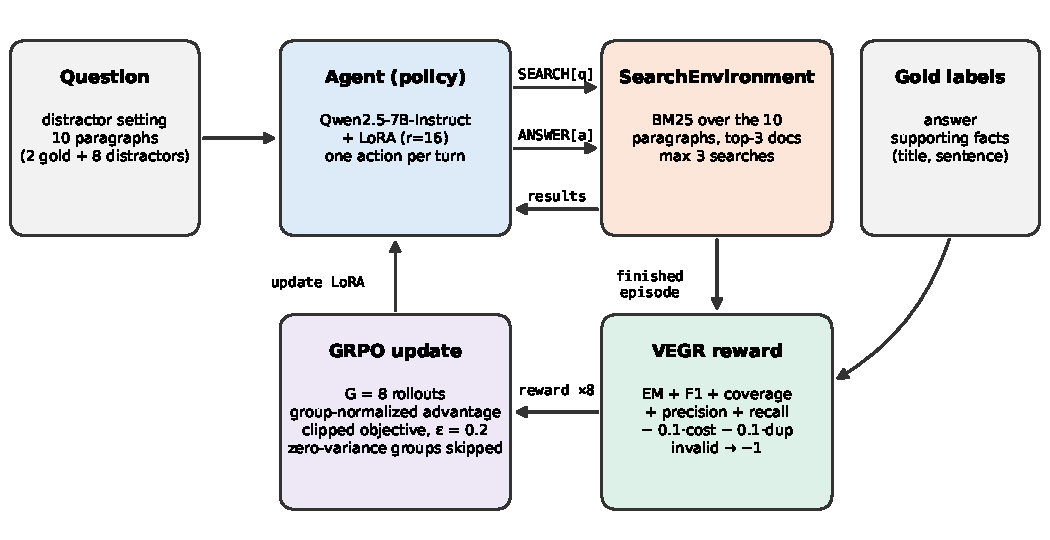
\includegraphics[keepaspectratio]{figures/fig3_1_system.pdf}}
\caption{One training step:}\label{fig:3.1}
\end{figure}

\begin{enumerate}
\def\labelenumi{\arabic{enumi}.}
\tightlist
\item
  The agent receives a HotpotQA question and takes up to 3
  \texttt{SEARCH} actions over the question's 10 paragraphs.
\item
  It ends with \texttt{ANSWER{[}a{]} CITATIONS{[}title|index; …{]}}.
\item
  The finished episode is scored by VEGR against the gold answer and
  supporting facts.
\item
  GRPO compares the rewards of 8 such episodes on the same question and
  updates the LoRA adapter.
\end{enumerate}

Drawn by
\texttt{scripts/\allowbreak{}make\_\allowbreak{}thesis\_\allowbreak{}figures.\allowbreak{}py}.

Three research questions guide the design (Chapter~\ref{sec:1}):

\begin{itemize}
\tightlist
\item
  \textbf{RQ1}: Does GRPO improve a 7B search agent over the un-tuned
  model?
\item
  \textbf{RQ2}: Does VEGR prevent the shortcut behaviour of answer-only
  reward, without losing accuracy?
\item
  \textbf{RQ3}: How do reward variants and optimizer fixes affect
  grounding and search behaviour?
\end{itemize}

\section{Dataset and splits}\label{sec:3.2}

The study uses \textbf{HotpotQA} (Yang et al., 2018), version 1.1, in
the \emph{distractor} setting. Each question comes with 10 Wikipedia
paragraphs: 2 gold paragraphs that contain the answer evidence, and 8
distractors. Each question is also annotated with \textbf{supporting
facts}, the (title, sentence index) pairs needed to answer it. These
annotations are what make a judge-free evidence reward possible: whether
a citation is correct can be checked by rule.

Rows that fail validation are skipped and logged with a reason (for
example, an empty sentence or a supporting-fact index out of range).

\textbf{Splits.} The split is produced by
\texttt{scripts/\allowbreak{}prepare\_\allowbreak{}splits.\allowbreak{}py}
and recorded in
\texttt{configs/\allowbreak{}evaluation/\allowbreak{}splits.\allowbreak{}json},
together with SHA-256 hashes of the source files.

\begin{itemize}
\tightlist
\item
  \textbf{Train / validation.} These are both drawn from the HotpotQA
  training file using a deterministic hash. Each question ID is mapped
  to a bucket in {[}0, 1) by taking the first 8 bytes of
  \texttt{sha256("7:" + question\_\allowbreak{}id)}. A question goes to
  train if the bucket is below 0.95, and to validation otherwise. This
  gives \textbf{85,573 training} and \textbf{4,452 validation}
  questions. The split does not depend on file order and can be
  reproduced exactly.
\item
  \textbf{Holdout.} The holdout is a frozen set of \textbf{300
  questions}: the first 300 valid rows of the HotpotQA dev file, stored
  in
  \texttt{configs/\allowbreak{}evaluation/\allowbreak{}holdout\_\allowbreak{}v1\_\allowbreak{}ids.\allowbreak{}json}
  along with a hash of the manifest. The holdout was never used to
  choose settings. All settings were chosen on the validation split, and
  the holdout is used only for the final numbers reported in
  Chapter~\ref{sec:4}.
\end{itemize}

\textbf{Training sample.} Each training run draws \textbf{256 questions}
from the training split. The sample depends on the run seed, so
different seeds see different questions (Section~\ref{sec:3.6}).

\section{Search environment}\label{sec:3.3}

The environment (\texttt{SearchEnvironment},
\texttt{src/\allowbreak{}needle/\allowbreak{}environment/\allowbreak{}search.\allowbreak{}py})
is a bounded, resettable search session over a single question.

\textbf{Corpus and retriever.} The searchable corpus is the question's
own 10 paragraphs. Retrieval uses Okapi BM25 (Robertson \& Zaragoza,
2009), via the \texttt{rank\_\allowbreak{}bm25} implementation with its
default parameters. Each paragraph is indexed as its title plus all its
sentences, tokenized into case-folded Unicode word tokens. A search
returns the \textbf{top 3} documents. Ties are broken by original
document order, so retrieval is deterministic. Each returned document is
shown in full, with numbered sentences.

\textbf{Budget.} An episode allows at most \textbf{3 searches}.

\textbf{Action grammar.} On each turn the agent must output exactly one
action:

\begin{itemize}
\tightlist
\item
  \texttt{SEARCH{[}query{]}} runs a BM25 search and spends one unit of
  budget.
\item
  \texttt{ANSWER{[}answer{]} CITATIONS{[}title|index; title|index; .\allowbreak{}.\allowbreak{}.\allowbreak{}{]}}
  gives the final answer together with the cited evidence sentences.
  This action ends the episode.
\end{itemize}

\textbf{Validation and failure types.} An episode is \textbf{invalid} if
any of the following happens:

\begin{itemize}
\tightlist
\item
  \emph{Protocol failure}: the output does not match the grammar (for
  example, extra text, or citations attached to a SEARCH action).
\item
  \emph{Evidence failure}: a citation refers to a title or sentence
  index that never appeared in any search result in the episode. In
  practice this mostly means invented citations.
\item
  \emph{Budget failure}: the agent uses all its searches and still does
  not answer.
\end{itemize}

Invalid episodes receive the protocol penalty of −1 during training
(Section~\ref{sec:3.4}) and count as wrong during evaluation
(Section~\ref{sec:3.7}).

\textbf{Known loophole.} An answer with an empty citation list
(\texttt{ANSWER{[}x{]}} or \texttt{ANSWER{[}x{]} CITATIONS{[}{]}}) is
accepted as valid. The prompt itself allows \texttt{CITATIONS{[}{]}} for
the case where no citation can be validated. We did not close this
loophole, so that every run is trained and evaluated in the same
environment. Chapter~\ref{sec:4} reports how the answer-only reward
exploited it.

\section{Proposed reward: VEGR}\label{sec:3.4}

The \textbf{Verifiable Evidence-Grounded Reward (VEGR)} is implemented
in
\texttt{src/\allowbreak{}needle/\allowbreak{}rewards/\allowbreak{}\_\allowbreak{}\_\allowbreak{}init\_\allowbreak{}\_\allowbreak{}.\allowbreak{}py}.
Every term is computed by rule from HotpotQA's gold annotations, so no
LLM judge is involved.

Let \emph{G} be the set of gold supporting facts (title, sentence index)
and \emph{C} the set of sentences the agent cites. For a valid episode:

\[
R_{\text{VEGR}} = \text{EM} + \text{F1} + \text{Cov} + \text{Prec} + \text{RetR} - 0.1\cdot\text{Cost} - 0.1\cdot\text{Dup}
\]

{\def\LTcaptype{none} % do not increment counter
\begin{longtable}[]{@{}
  >{\raggedright\arraybackslash}p{(\linewidth - 4\tabcolsep) * \real{0.3333}}
  >{\raggedright\arraybackslash}p{(\linewidth - 4\tabcolsep) * \real{0.3333}}
  >{\raggedright\arraybackslash}p{(\linewidth - 4\tabcolsep) * \real{0.3333}}@{}}
\toprule\noalign{}
\begin{minipage}[b]{\linewidth}\raggedright
Term
\end{minipage} & \begin{minipage}[b]{\linewidth}\raggedright
Definition
\end{minipage} & \begin{minipage}[b]{\linewidth}\raggedright
Range
\end{minipage} \\
\midrule\noalign{}
\endhead
\bottomrule\noalign{}
\endlastfoot
EM & normalized exact match between predicted and gold answer & \{0,
1\} \\
F1 & token-level F1 between predicted and gold answer & {[}0, 1{]} \\
Cov (evidence coverage) & \textbar G ∩ C\textbar{} /
\textbar G\textbar{} & {[}0, 1{]} \\
Prec (citation precision) & \textbar G ∩ C\textbar{} /
\textbar C\textbar, defined as 0 when C is empty & {[}0, 1{]} \\
RetR (retrieval recall) & fraction of gold documents that appeared in
any search result & {[}0, 1{]} \\
Cost (search cost) & searches used / budget (3) & {[}0, 1{]} \\
Dup (duplicate-query penalty) & (number of queries − number of unique
queries) / number of queries & {[}0, 1) \\
\end{longtable}
}

An \textbf{invalid} episode receives \textbf{R = −1}, regardless of the
other terms. This protocol penalty is what makes VEGR enforce the action
grammar. Because an invented citation is an evidence failure, the agent
cannot raise its precision by citing sentences it never retrieved.

The terms fall into three groups, each aimed at a different failure:

\begin{itemize}
\tightlist
\item
  \textbf{Answer terms (EM, F1)} reward correctness. F1 gives partial
  credit, so the reward is less sparse than EM alone.
\item
  \textbf{Evidence terms (Cov, Prec)} reward citing the right sentences.
  Precision alone could be satisfied by citing a single safe sentence,
  and coverage alone by citing everything, so both are included
  (cf.~ALCE; Gao et al., 2023).
\item
  \textbf{Search terms (RetR, Cost, Dup)} reward finding the gold
  documents and penalize wasted or repeated searches. The penalties have
  a small weight (0.1) so that they shape search behaviour without
  discouraging search altogether.
\end{itemize}

The individual terms are not new. The contribution is combining them
into a judge-free reward for multi-turn search agents, together with a
controlled evaluation of what the combination changes
(Section~\ref{sec:3.8}). All weights are untuned defaults. This is a
limitation, discussed in Chapter~\ref{sec:5}.

\textbf{Worked example.} Table~\ref{tbl:3.1} scores two real holdout
episodes for the same question (\texttt{5abd94525542992ac4f382d2},
``Which company formed the boy group that debuted with \emph{2014
S/S}?''). Both answer ``YG Entertainment'' correctly. Under the
outcome-only reward (R0) both receive the same reward, 1. VEGR separates
them: one is fully grounded, the other has no evidence.

\begin{longtable}[]{@{}
  >{\raggedright\arraybackslash}p{(\linewidth - 4\tabcolsep) * \real{0.3333}}
  >{\raggedright\arraybackslash}p{(\linewidth - 4\tabcolsep) * \real{0.3333}}
  >{\raggedright\arraybackslash}p{(\linewidth - 4\tabcolsep) * \real{0.3333}}@{}}
\caption{VEGR terms for two correct answers to the same question. Values
are taken from
\texttt{results/\allowbreak{}2026-\allowbreak{}10-\allowbreak{}10-\allowbreak{}batch/\allowbreak{}\{r1\_\allowbreak{}full\_\allowbreak{}seed8,r0\_\allowbreak{}outcome\_\allowbreak{}seed8\}/\allowbreak{}episodes.\allowbreak{}jsonl}.}\label{tbl:3.1}\tabularnewline
\toprule\noalign{}
\begin{minipage}[b]{\linewidth}\raggedright
\end{minipage} & \begin{minipage}[b]{\linewidth}\raggedright
Episode A (R1 seed 8)
\end{minipage} & \begin{minipage}[b]{\linewidth}\raggedright
Episode B (R0 seed 8)
\end{minipage} \\
\midrule\noalign{}
\endfirsthead
\toprule\noalign{}
\begin{minipage}[b]{\linewidth}\raggedright
\end{minipage} & \begin{minipage}[b]{\linewidth}\raggedright
Episode A (R1 seed 8)
\end{minipage} & \begin{minipage}[b]{\linewidth}\raggedright
Episode B (R0 seed 8)
\end{minipage} \\
\midrule\noalign{}
\endhead
\bottomrule\noalign{}
\endlastfoot
Actions &
\texttt{SEARCH{[}S/\allowbreak{}S 2014 debut South Korean boy group{]}}
→ \texttt{SEARCH{[}WINNER YG Entertainment{]}} →
\texttt{ANSWER{[}YG Entertainment{]} CITATIONS{[}2014 S/\allowbreak{}S\textbackslash{}|0; Winner (band)\textbackslash{}|0{]}}
&
\texttt{SEARCH{[}2014 S/\allowbreak{}S debut album South Korean boy group formed by{]}}
→ \texttt{ANSWER{[}YG Entertainment{]}} \\
EM & 1 & 1 \\
F1 & 1 & 1 \\
Evidence coverage & 1 (both gold sentences cited) & 0 (nothing cited) \\
Citation precision & 1 & 0 \\
Retrieval recall & 1 (both gold documents retrieved) & 0.5 (one of
two) \\
− 0.1 · search cost & − 0.1 · 2/3 = − 0.067 & − 0.1 · 1/3 = − 0.033 \\
− 0.1 · duplicate penalty & 0 & 0 \\
\textbf{VEGR total} & \textbf{4.933} & \textbf{2.467} \\
Outcome-only reward (R0) & 1 & 1 \\
\end{longtable}

\textbf{Reward variants.} Three variants change one aspect of VEGR at a
time:

\begin{itemize}
\tightlist
\item
  \textbf{R0, outcome-only (baseline reward).} R = EM. All other weights
  are 0, but invalid episodes still receive −1. This mirrors
  outcome-reward search agents such as Search-R1 (Jin et al., 2025).
\item
  \textbf{R2, gated penalties.} This is VEGR, except that the
  search-cost and duplicate penalties apply only when EM = 1. The idea
  is to avoid penalizing search on questions the agent has not yet
  solved.
\item
  \textbf{R3, coverage ×2.} This is VEGR with the evidence-coverage
  weight raised from 1 to 2. It targets the ``precise but incomplete''
  citation pattern described in Chapter~\ref{sec:4}.
\end{itemize}

\section{Policy model}\label{sec:3.5}

\textbf{Base model.} The policy is \textbf{Qwen2.5-7B-Instruct} (Qwen
Team, 2024), loaded from local weights in bf16.

\textbf{Prompt.} The prompt is deterministic and built by
\texttt{build\_\allowbreak{}prompt} in
\texttt{src/\allowbreak{}needle/\allowbreak{}inference/\allowbreak{}runner.\allowbreak{}py}.
It is wrapped in the model's chat template. The prompt:

\begin{enumerate}
\def\labelenumi{\arabic{enumi}.}
\tightlist
\item
  Describes the role (``You are a careful evidence-seeking QA agent'').
\item
  States the action grammar, gives a worked example
  (\texttt{ANSWER{[}United States{]} CITATIONS{[}Ursula K.\allowbreak{} Le Guin|1; The Left Hand of Darkness|1{]}}),
  and lists formatting rules: one \texttt{title|index} per citation,
  semicolon-separated, no text after the closing bracket, titles copied
  exactly, never invent a title.
\item
  Gives the question and the remaining search budget.
\item
  Lists all search results so far. For each search, it shows the query
  and then every returned document as \texttt{{[}Title{]}} followed by
  \texttt{index: sentence} lines.
\end{enumerate}

The prompt is rebuilt from scratch every turn, so the model always sees
the full search history. Appendix A gives the complete prompt for one
real holdout question, at the point just before the agent gives its
final answer.

\textbf{Adapter.} Training uses LoRA (Hu et al., 2022) with rank r = 16,
α = 32, and dropout 0. The adapter is applied to all attention and MLP
projections (q, k, v, o, gate, up, down). The base weights stay frozen,
which makes training on a single 48 GB GPU possible.

\section{Training algorithm}\label{sec:3.6}

Training uses \textbf{Group Relative Policy Optimization} (GRPO; Shao et
al., 2024), extended to multi-turn episodes. The implementation is in
\texttt{scripts/\allowbreak{}train\_\allowbreak{}grpo.\allowbreak{}py}
and
\texttt{src/\allowbreak{}needle/\allowbreak{}training/\allowbreak{}grpo.\allowbreak{}py}.

\textbf{Rollouts.} For each training question, the current policy runs
\textbf{G = 8} full episodes, sampling with temperature 1.0 and top-p
1.0. Each action is limited to 128 new tokens. Each episode receives one
scalar reward from the reward function of the run (R0--R3).

\textbf{Advantage.} Each reward is normalized within its group:

\[
A_i = \frac{r_i - \operatorname{mean}(r_{1..G})}{\operatorname{std}(r_{1..G}) + 10^{-6}}
\]

All actions in an episode share the episode's advantage. If all 8
rewards in a group are equal, every advantage is zero and the group
carries no learning signal. Such \textbf{zero-variance groups are
skipped}: no update is made. The number of skipped steps is logged, and
it turns out to be an important diagnostic (Chapter~\ref{sec:4}).

\textbf{Objective.} The update uses the PPO-style clipped surrogate
(Schulman et al., 2017) with ε = 0.2. Each rollout's log-probability is
the \textbf{mean over all tokens the agent generated in that episode},
across all its actions. Prompt and observation tokens are excluded. The
ratio ρ is therefore computed once per rollout.

\[
\mathcal{L} = -\,\mathbb{E}\left[\min\left(\rho\,A,\; \operatorname{clip}(\rho,\,1-\varepsilon,\,1+\varepsilon)\,A\right)\right],
\qquad \rho = \exp\left(\log\pi_\theta - \log\pi_{\theta_\text{old}}\right)
\]

There is \textbf{no KL penalty} to a reference model. Invalid rollouts
stay in the batch, so the −1 penalty actively pushes the policy away
from malformed actions.

\textbf{Optimization.} AdamW with learning rate 2 × 10⁻⁵, gradient-norm
clipping at 1.0, bf16, and gradient checkpointing. A run makes one pass
over its 256 questions (256 steps, one question per step).

\textbf{Seeds.} Runs use seeds 7, 8, and 9. A seed fixes both the
256-question training sample and the random state used for sampling
rollouts. Seed-to-seed differences therefore reflect both data and
optimization noise.

\textbf{Optimizer variants.} Two variants change the optimizer instead
of the reward:

\begin{itemize}
\tightlist
\item
  \textbf{Dr.~GRPO advantages} (Liu et al., 2025), used in R4. The
  advantage is computed without dividing by the standard deviation, A\_i
  = r\_i − mean(r). This removes the scaling that amplifies groups whose
  rewards are nearly equal.
\item
  \textbf{DAPO-style dynamic sampling} (Yu et al., 2025), used in
  R0-dyn. Zero-variance groups do not count toward the step budget. The
  trainer keeps drawing questions, from a pool of up to 512, until it
  has made 256 actual optimizer updates. This tests whether R0's
  shortcut comes from having too few informative updates.
\end{itemize}

\textbf{Pseudocode.}

\begin{Verbatim}
for step, question in enumerate(sample(train_split, 256, seed)):
    episodes = [run_episode(policy, question) for _ in range(8)]   # multi-turn
    rewards  = [reward_fn(ep, gold(question)) for ep in episodes]  # VEGR or variant; invalid → −1
    if all rewards equal:
        log_skip(step); continue                                    # zero-variance group
    A = (rewards − mean(rewards)) / (std(rewards) + 1e-6)          # Dr. GRPO: no division
    for each episode i:
        ρ = exp(mean_token_logp_θ(actions_i) − mean_token_logp_old(actions_i))  # mean over all action tokens
        loss += −min(ρ·A_i, clip(ρ, 0.8, 1.2)·A_i)
    update LoRA with AdamW (lr 2e-5, grad clip 1.0)
\end{Verbatim}

\section{Evaluation protocol}\label{sec:3.7}

\textbf{Setting.} Every model is evaluated on the same frozen
\textbf{300-question holdout}, with greedy decoding and \textbf{no
retries}. If an action is malformed, the episode fails.

\textbf{Metrics.}

\begin{itemize}
\tightlist
\item
  \textbf{EM (all)} is the headline accuracy number. Every invalid
  episode counts as 0, so the denominator is always 300.
\item
  \textbf{Completed episodes} is the number of valid episodes out of
  300. Failures are broken down by type (evidence, protocol, budget).
\item
  \textbf{Quality metrics} are F1, evidence coverage, citation
  precision, retrieval recall, and searches per episode. Each is
  averaged over completed episodes only, using the definitions in
  Section~\ref{sec:3.4}.
\item
  \textbf{Grounded EM} counts an episode only if EM = 1, it has at least
  one citation, and every citation is a gold supporting fact. This is a
  strict metric: a correct answer with one non-gold citation does not
  count. It is the measure most directly tied to the thesis claim that
  answers should be correct \emph{and} supported by evidence.
\item
  \textbf{Behavioural diagnostics} come from the episode and training
  logs. They include the share of episodes that repeat a query, the
  distribution of citation counts and cited sentence indices, the
  invalid rate during training, and the number of skipped
  (zero-variance) training steps.
\end{itemize}

\textbf{Statistics.} Following Agarwal et al.~(2021) and Henderson et
al.~(2018), single runs are not treated as conclusive.

\begin{itemize}
\tightlist
\item
  Differences in EM between two models are tested with a \textbf{paired
  bootstrap} over the 300 holdout questions: 10,000 resamples and a 95\%
  percentile confidence interval. A difference is called significant
  only if the CI excludes 0.
\item
  Each reward variant is trained with \textbf{3 seeds} (7, 8, 9).
  Results are reported per seed and as the mean across seeds.
\item
  Since seeds of the same method can differ by several EM points, a
  method difference is only claimed when it holds across seeds, not when
  it shows up for a single seed.
\end{itemize}

\section{Experiment matrix}\label{sec:3.8}

{\def\LTcaptype{none} % do not increment counter
\begin{longtable}[]{@{}
  >{\raggedright\arraybackslash}p{(\linewidth - 8\tabcolsep) * \real{0.2000}}
  >{\raggedright\arraybackslash}p{(\linewidth - 8\tabcolsep) * \real{0.2000}}
  >{\raggedright\arraybackslash}p{(\linewidth - 8\tabcolsep) * \real{0.2000}}
  >{\raggedright\arraybackslash}p{(\linewidth - 8\tabcolsep) * \real{0.2000}}
  >{\raggedright\arraybackslash}p{(\linewidth - 8\tabcolsep) * \real{0.2000}}@{}}
\toprule\noalign{}
\begin{minipage}[b]{\linewidth}\raggedright
ID
\end{minipage} & \begin{minipage}[b]{\linewidth}\raggedright
Name
\end{minipage} & \begin{minipage}[b]{\linewidth}\raggedright
Reward
\end{minipage} & \begin{minipage}[b]{\linewidth}\raggedright
Optimizer
\end{minipage} & \begin{minipage}[b]{\linewidth}\raggedright
Seeds
\end{minipage} \\
\midrule\noalign{}
\endhead
\bottomrule\noalign{}
\endlastfoot
B0 & Un-tuned baseline & --- (no training) & --- & --- \\
R0 & Outcome-only & EM, invalid −1 & GRPO & 7, 8, 9 \\
R1 & \textbf{VEGR} & full VEGR & GRPO & 7, 8, 9 \\
R2 & Gated & VEGR, penalties only when EM = 1 & GRPO & 7, 8, 9 \\
R3 & Coverage ×2 & VEGR, coverage weight 2 & GRPO & 7, 8, 9 \\
R4 & VEGR + Dr.~GRPO & full VEGR & GRPO, no std division & 7, 8, 9 \\
R0-dyn & Outcome-only + dynamic sampling & EM, invalid −1 & GRPO + DAPO
dynamic sampling & 8 \\
\end{longtable}
}

The comparisons map onto the research questions:

\begin{itemize}
\tightlist
\item
  \textbf{RQ1:} every trained run against B0.
\item
  \textbf{RQ2:} R1 against R0. Same optimizer, same seeds, different
  reward.
\item
  \textbf{RQ3:}

  \begin{itemize}
  \tightlist
  \item
    R2 and R3 against R1 test reward design.
  \item
    R4 against R1, and R0-dyn against R0, test optimizer fixes.
  \item
    R0-dyn is the key control. If dynamic sampling alone removes R0's
    shortcut, the problem was the optimizer and not the reward. If it
    does not, the evidence reward is necessary.
  \end{itemize}
\end{itemize}

R0-dyn was run on a single seed (seed 8) as a \textbf{diagnostic
experiment}, not as one of the main methods.

\begin{itemize}
\tightlist
\item
  \textbf{Why one seed (cost).} Dynamic sampling discards zero-variance
  groups, and R0 seed 8 skipped 128 of its 256 steps. Reaching 256 real
  updates is therefore expected to take up to about 512 questions,
  roughly twice the rollouts and cost of a standard run. The budget
  extension originally planned this test on two seeds. It was cut to one
  so that the 3-seed runs of the main methods (R0--R4) fit the budget.
  {[}TODO: replace ``expected'' with the actual number of questions
  drawn and the run time.{]}
\item
  \textbf{Why seed 8.} It is the seed on which outcome-only training
  collapsed to uncited answers. The question is narrow: does an
  optimizer-level fix alone prevent this shortcut where it actually
  happened? A seed on which R0 did not collapse could not answer that.
\item
  \textbf{How it is read.} R0-dyn is interpreted as a case study about
  mechanism, not as a statistically supported comparison between
  methods.
\end{itemize}

\textbf{Planned vs.~post hoc.} B0, R0, R1, and R2 were specified before
the multi-seed batch ran
(\texttt{logs/\allowbreak{}2026-\allowbreak{}10-\allowbreak{}10-\allowbreak{}r0-\allowbreak{}r1-\allowbreak{}r2-\allowbreak{}batch.\allowbreak{}md}).
Only the single R1 seed-7 run existed at that point. R3, R4, and R0-dyn
were added on 2026-10-11, after the R0/R1/R2 results had been analysed
(\texttt{docs/\allowbreak{}research/\allowbreak{}2026-\allowbreak{}10-\allowbreak{}11-\allowbreak{}results-\allowbreak{}diagnosis-\allowbreak{}and-\allowbreak{}improvements.\allowbreak{}md}).
They respond to specific observations: low evidence coverage, and R0's
skipped steps and shortcuts. They are therefore \textbf{exploratory
follow-ups}, and Chapter~\ref{sec:4} reports them as such rather than as
confirmatory tests.

\section{Implementation and compute}\label{sec:3.9}

\textbf{Software.} Python 3.11 (managed with \texttt{uv}), Transformers
4.57.6, PEFT 0.21.2, and \texttt{rank\_\allowbreak{}bm25}. PyTorch
differs between runs:

\begin{itemize}
\tightlist
\item
  The first runs (B0 and R1 seed 7) used \textbf{2.14.1+cu130}.
\item
  All later runs used \textbf{2.11.0+cu128}, because the later pod's GPU
  driver supported only CUDA 12.8.
\end{itemize}

This is reported as a limitation when comparing against R1 seed 7.
Training and evaluation run offline from local weights, with Hugging
Face offline mode on.

\textbf{Hardware and cost.} One NVIDIA L40S (48 GB) on RunPod at about
\$1.10 per hour. One run (training plus holdout evaluation) takes about
2.05 hours, or roughly \textbf{\$2.25}. The total project budget is
about \$45. \texttt{{[}TODO: final cost table after the fixes batch{]}}

\textbf{Reproducibility.}

\begin{itemize}
\tightlist
\item
  Splits are fixed by hashed manifests (Section~\ref{sec:3.2}).
\item
  Every run is defined by a JSON config in
  \texttt{configs/\allowbreak{}training/\allowbreak{}} and writes
  \texttt{run\_\allowbreak{}metadata.\allowbreak{}json} (library
  versions, seed, config), \texttt{summary.\allowbreak{}json},
  \texttt{episodes.\allowbreak{}jsonl} (every evaluation episode), and
  \texttt{metrics.\allowbreak{}jsonl} (per-step training metrics) to
  \texttt{results/\allowbreak{}<date>/\allowbreak{}<run>/\allowbreak{}}.
\item
  Each batch has a dated log in \texttt{logs/\allowbreak{}}.
\item
  The step-by-step procedure for reproducing the runs on RunPod is in
  \texttt{docs/\allowbreak{}runbooks/\allowbreak{}runpod.\allowbreak{}md}.
\end{itemize}

\begin{center}\rule{0.5\linewidth}{0.5pt}\end{center}

\section{Provenance (remove before
submission)}\label{provenance-remove-before-submission}

{\def\LTcaptype{none} % do not increment counter
\begin{longtable}[]{@{}
  >{\raggedright\arraybackslash}p{(\linewidth - 2\tabcolsep) * \real{0.5000}}
  >{\raggedright\arraybackslash}p{(\linewidth - 2\tabcolsep) * \real{0.5000}}@{}}
\toprule\noalign{}
\begin{minipage}[b]{\linewidth}\raggedright
Claim in this chapter
\end{minipage} & \begin{minipage}[b]{\linewidth}\raggedright
Source
\end{minipage} \\
\midrule\noalign{}
\endhead
\bottomrule\noalign{}
\endlastfoot
Split algorithm, 0.95 fraction, 85,573 / 4,452 counts, holdout = first
300 valid dev rows &
\texttt{configs/\allowbreak{}evaluation/\allowbreak{}splits.\allowbreak{}json},
\texttt{scripts/\allowbreak{}prepare\_\allowbreak{}splits.\allowbreak{}py} \\
BM25 (\texttt{rank\_\allowbreak{}bm25.\allowbreak{}BM25Okapi},
defaults), tokenizer, tie-breaking &
\texttt{src/\allowbreak{}needle/\allowbreak{}retrieval/\allowbreak{}bm25.\allowbreak{}py} \\
Top-k 3, budget 3, failure types, no-citation loophole & writer brief
§3;
\texttt{src/\allowbreak{}needle/\allowbreak{}environment/\allowbreak{}search.\allowbreak{}py} \\
Prompt content, chat template &
\texttt{src/\allowbreak{}needle/\allowbreak{}inference/\allowbreak{}runner.\allowbreak{}py::build\_\allowbreak{}prompt};
\texttt{src/\allowbreak{}needle/\allowbreak{}training/\allowbreak{}local\_\allowbreak{}policy.\allowbreak{}py} \\
Reward formula and weights &
\texttt{src/\allowbreak{}needle/\allowbreak{}rewards/\allowbreak{}\_\allowbreak{}\_\allowbreak{}init\_\allowbreak{}\_\allowbreak{}.\allowbreak{}py};
writer brief §3 \\
GRPO settings, per-rollout sequence-mean ratio, clipping &
\texttt{src/\allowbreak{}needle/\allowbreak{}training/\allowbreak{}grpo.\allowbreak{}py},
\texttt{scripts/\allowbreak{}train\_\allowbreak{}grpo.\allowbreak{}py} \\
Dynamic sampling (512 pool, 256 updates) &
\texttt{logs/\allowbreak{}2026-\allowbreak{}10-\allowbreak{}11-\allowbreak{}fixes-\allowbreak{}batch.\allowbreak{}md} \\
Library versions, torch change and reason &
\texttt{results/\allowbreak{}*/\allowbreak{}run\_\allowbreak{}metadata.\allowbreak{}json};
\texttt{logs/\allowbreak{}2026-\allowbreak{}10-\allowbreak{}10-\allowbreak{}r0-\allowbreak{}r1-\allowbreak{}r2-\allowbreak{}batch.\allowbreak{}md} \\
Cost per run, budget & writer brief §3;
\texttt{logs/\allowbreak{}2026-\allowbreak{}10-\allowbreak{}11-\allowbreak{}fixes-\allowbreak{}batch.\allowbreak{}md} \\
\texttt{uv} & \texttt{uv.\allowbreak{}lock} in repo root \\
\end{longtable}
}

\chapter{Results and Discussion}\label{sec:4}

\begin{quote}
\textbf{DRAFT --- not submission-ready.} Status as of 2026-10-11. Every
number comes from
\texttt{docs/\allowbreak{}thesis/\allowbreak{}writer-\allowbreak{}brief.\allowbreak{}md}
§4 or from
\texttt{results/\allowbreak{}2026-\allowbreak{}10-\allowbreak{}10-\allowbreak{}batch/\allowbreak{}*/\allowbreak{}episodes.\allowbreak{}jsonl}.
Results from the fixes batch (R0 seed 9, R3, R4, R0-dyn), grounded EM,
and the seed-9 confidence intervals are \textbf{pending} (expected
\textasciitilde12:30 WIB 2026-10-12, in
\texttt{logs/\allowbreak{}2026-\allowbreak{}10-\allowbreak{}11-\allowbreak{}fixes-\allowbreak{}batch.\allowbreak{}md}).
They are marked \texttt{{[}TODO{]}}. This chapter reports the results in
the order of the research questions:
\end{quote}

\begin{itemize}
\tightlist
\item
  \textbf{4.1} gives the experimental setup.
\item
  \textbf{4.2} describes the un-tuned baseline.
\item
  \textbf{4.3 to 4.6} answer RQ1, RQ2 and RQ3, with a diagnosis of
  training dynamics in between (4.5).
\item
  \textbf{4.7} shows example traces.
\item
  \textbf{4.8} discusses the findings and threats to validity.
\end{itemize}

Throughout, \textbf{EM (all)} is the headline accuracy number: invalid
episodes count as wrong, so the denominator is always 300. Quality
metrics (F1, coverage, precision, recall, searches) are averaged over
\textbf{completed} episodes only (Section~\ref{sec:3.7}).

\section{Experimental setup}\label{sec:4.1}

{\def\LTcaptype{none} % do not increment counter
\begin{longtable}[]{@{}
  >{\raggedright\arraybackslash}p{(\linewidth - 2\tabcolsep) * \real{0.5000}}
  >{\raggedright\arraybackslash}p{(\linewidth - 2\tabcolsep) * \real{0.5000}}@{}}
\toprule\noalign{}
\begin{minipage}[b]{\linewidth}\raggedright
Setting
\end{minipage} & \begin{minipage}[b]{\linewidth}\raggedright
Value
\end{minipage} \\
\midrule\noalign{}
\endhead
\bottomrule\noalign{}
\endlastfoot
Model & Qwen2.5-7B-Instruct + LoRA (r = 16, α = 32) \\
Training data per run & 256 HotpotQA training questions (seed-dependent
sample), 1 epoch \\
Group size / learning rate & G = 8 / 2 × 10⁻⁵ \\
Search budget / top-k & 3 searches / 3 documents \\
Evaluation & 300-question frozen holdout, greedy decoding, no retries \\
Seeds & 7, 8, 9 \\
Hardware & 1 × NVIDIA L40S 48 GB (RunPod, \textasciitilde\$1.10/h) \\
Time and cost per run & ≈ 2.05 h ≈ \$2.25 (training + holdout
evaluation) \\
Total GPU hours and cost & {[}TODO: final cost table after the fixes
batch{]} \\
\end{longtable}
}

\section{Baseline (B0)}\label{sec:4.2}

The un-tuned model reaches \textbf{22.3\% EM} on the holdout. Its main
problem is not wrong answers but invalid episodes: only \textbf{170 of
300} episodes complete. The 130 failures break down into 85 evidence
failures, 37 protocol failures, and 8 budget failures. Most evidence
failures are invented or unretrievable citations, meaning the model
cites a title or sentence it never retrieved.

When the model does complete an episode, it is reasonably capable. EM
over completed episodes is 39.4\%, citation precision 0.633, and
retrieval recall 0.829 (Table~\ref{tbl:4.1}). This already suggests that
much of what training can gain lies in following the protocol, which
Section~\ref{sec:4.3} confirms.

\section{RQ1: Does GRPO improve the agent over the un-tuned
model?}\label{sec:4.3}

\begin{longtable}[]{@{}
  >{\raggedright\arraybackslash}p{(\linewidth - 16\tabcolsep) * \real{0.1111}}
  >{\raggedright\arraybackslash}p{(\linewidth - 16\tabcolsep) * \real{0.1111}}
  >{\raggedright\arraybackslash}p{(\linewidth - 16\tabcolsep) * \real{0.1111}}
  >{\raggedright\arraybackslash}p{(\linewidth - 16\tabcolsep) * \real{0.1111}}
  >{\raggedright\arraybackslash}p{(\linewidth - 16\tabcolsep) * \real{0.1111}}
  >{\raggedright\arraybackslash}p{(\linewidth - 16\tabcolsep) * \real{0.1111}}
  >{\raggedright\arraybackslash}p{(\linewidth - 16\tabcolsep) * \real{0.1111}}
  >{\raggedright\arraybackslash}p{(\linewidth - 16\tabcolsep) * \real{0.1111}}
  >{\raggedright\arraybackslash}p{(\linewidth - 16\tabcolsep) * \real{0.1111}}@{}}
\caption{Holdout results. EM (all) counts failures as 0; other columns
are means over completed episodes.}\label{tbl:4.1}\tabularnewline
\toprule\noalign{}
\begin{minipage}[b]{\linewidth}\raggedright
Run
\end{minipage} & \begin{minipage}[b]{\linewidth}\raggedright
Seed
\end{minipage} & \begin{minipage}[b]{\linewidth}\raggedright
EM (all)
\end{minipage} & \begin{minipage}[b]{\linewidth}\raggedright
Completed /300
\end{minipage} & \begin{minipage}[b]{\linewidth}\raggedright
F1
\end{minipage} & \begin{minipage}[b]{\linewidth}\raggedright
Evid. cov.
\end{minipage} & \begin{minipage}[b]{\linewidth}\raggedright
Cit. prec.
\end{minipage} & \begin{minipage}[b]{\linewidth}\raggedright
Retr. recall
\end{minipage} & \begin{minipage}[b]{\linewidth}\raggedright
Searches
\end{minipage} \\
\midrule\noalign{}
\endfirsthead
\toprule\noalign{}
\begin{minipage}[b]{\linewidth}\raggedright
Run
\end{minipage} & \begin{minipage}[b]{\linewidth}\raggedright
Seed
\end{minipage} & \begin{minipage}[b]{\linewidth}\raggedright
EM (all)
\end{minipage} & \begin{minipage}[b]{\linewidth}\raggedright
Completed /300
\end{minipage} & \begin{minipage}[b]{\linewidth}\raggedright
F1
\end{minipage} & \begin{minipage}[b]{\linewidth}\raggedright
Evid. cov.
\end{minipage} & \begin{minipage}[b]{\linewidth}\raggedright
Cit. prec.
\end{minipage} & \begin{minipage}[b]{\linewidth}\raggedright
Retr. recall
\end{minipage} & \begin{minipage}[b]{\linewidth}\raggedright
Searches
\end{minipage} \\
\midrule\noalign{}
\endhead
\bottomrule\noalign{}
\endlastfoot
B0 & -- & 22.3\% & 170 & 0.501 & 0.472 & 0.633 & 0.829 & 1.92 \\
R0 & 7 & 42.0\% & 278 & 0.576 & 0.438 & 0.621 & 0.829 & 3.00 \\
R0 & 8 & 40.7\% & 299 & 0.530 & 0.000 & 0.000 & 0.710 & 1.01 \\
R0 & 9 & {[}TODO{]} & & & & & & \\
R1 (VEGR) & 7 & 42.7\% & 287 & 0.593 & 0.473 & 0.751 & 0.851 & 2.30 \\
R1 (VEGR) & 8 & 42.7\% & 287 & 0.574 & 0.513 & 0.726 & 0.836 & 2.15 \\
R1 (VEGR) & 9 & 45.3\% & 293 & 0.598 & 0.333 & 0.754 & 0.837 & 1.91 \\
R2 (gated) & 7 & 41.0\% & 283 & 0.577 & 0.539 & 0.748 & 0.891 & 2.21 \\
R2 (gated) & 8 & 48.7\% & 290 & 0.625 & 0.440 & 0.703 & 0.879 & 2.00 \\
R2 (gated) & 9 & 38.3\% & 286 & 0.552 & 0.471 & 0.702 & 0.855 & 2.16 \\
\end{longtable}

\begin{longtable}[]{@{}lll@{}}
\caption{Paired bootstrap on EM (10,000 resamples, 95\%
CI).}\label{tbl:4.2}\tabularnewline
\toprule\noalign{}
Comparison & ΔEM (points) & 95\% CI \\
\midrule\noalign{}
\endfirsthead
\toprule\noalign{}
Comparison & ΔEM (points) & 95\% CI \\
\midrule\noalign{}
\endhead
\bottomrule\noalign{}
\endlastfoot
R0 s7 − B0 & +19.7 & {[}+14.3, +25.0{]} \\
R0 s8 − B0 & +18.3 & {[}+13.3, +23.3{]} \\
R1 s7 − B0 & +20.3 & {[}+15.0, +25.7{]} \\
R1 s8 − B0 & +20.3 & {[}+15.3, +25.3{]} \\
R2 s7 − B0 & +18.7 & {[}+13.7, +24.0{]} \\
R2 s8 − B0 & +26.3 & {[}+21.0, +31.7{]} \\
Seed-9 comparisons & {[}TODO{]} & {[}TODO{]} \\
\end{longtable}

All intervals were recomputed from the per-question episode files with
\texttt{scripts/\allowbreak{}make\_\allowbreak{}thesis\_\allowbreak{}figures.\allowbreak{}py}
(10,000 resamples, fixed RNG seed 0). Compared with the earlier ad-hoc
computation, endpoints differ by at most 0.3 points, which is resampling
noise. Figure~\ref{fig:4.5} shows the same intervals, together with the
between-reward comparisons.

\begin{figure}
\centering
\pandocbounded{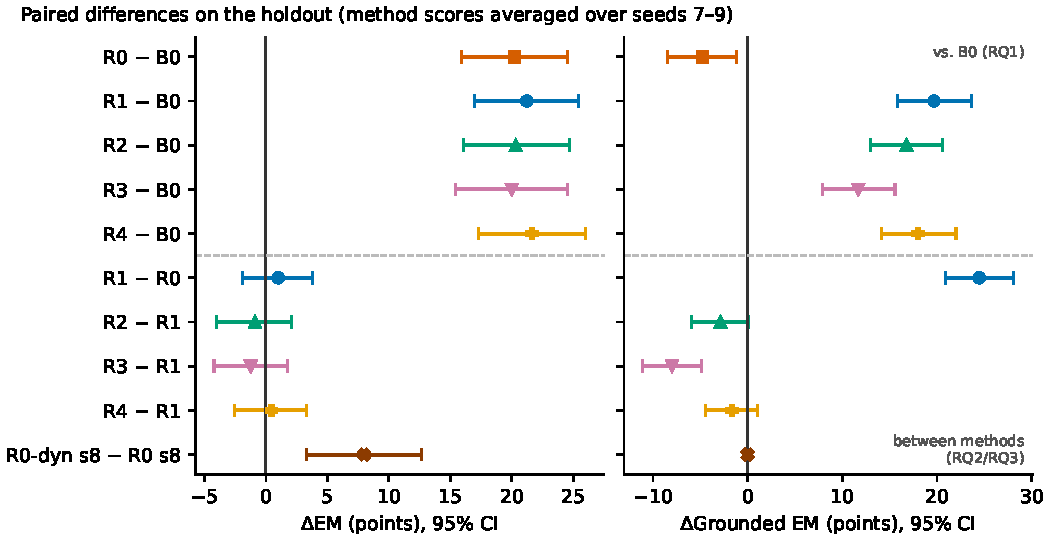
\includegraphics[keepaspectratio]{figures/fig4_5_bootstrap.pdf}}
\caption{Paired bootstrap differences in holdout EM, with 95\% CIs over
the 300 holdout questions.}\label{fig:4.5}
\end{figure}

\begin{itemize}
\tightlist
\item
  \textbf{Above the dashed line:} each trained run against B0 (RQ1).
  Every interval lies far to the right of zero.
\item
  \textbf{Below the dashed line:} comparisons between rewards on the
  same seed (RQ2/RQ3). Three of the four intervals cross zero. The
  exception, R2 s8 − R1 s8, does not replicate on other seeds
  (Section~\ref{sec:4.6}).
\end{itemize}

\textbf{Answer to RQ1: yes.} Every trained run with a computed CI beats
B0 by \textbf{+18.3 to +26.3 EM points}, and every confidence interval
excludes zero. The seed-9 runs (R1 45.3\%, R2 38.3\%) are also well
above B0's 22.3\%, but their CIs are not computed yet.

\textbf{Where the gain comes from.} Most of the improvement comes from
learning the protocol:

\begin{itemize}
\tightlist
\item
  B0 loses 130 of 300 episodes to failures, while every trained run in
  Table~\ref{tbl:4.1} loses at most 22.
\item
  Measured over completed episodes only, accuracy moves much less: from
  39.4\% (B0) to 44.6\% (R1 seed 7).
\end{itemize}

So GRPO mostly teaches the model to produce valid, verifiable actions,
and only modestly improves its reasoning on questions it could already
complete. The training logs of R1 seed 7 show this directly. The
invalid-rollout rate falls from 46\% to 29\%, 13\%, 13\% and 7\% over
the first five 32-step blocks, while average reward rises from 0.97 to
2.81.

\textbf{Validation split (supporting evidence only).} On the validation
split, R1 seed 7 reaches 57.0\% EM against B0's 29.3\% (+27.7 points,
95\% CI {[}+21.7, +33.7{]}). The validation questions appear easier than
the holdout, so this number is not used for any claim. It only shows
that the gain is not specific to the holdout.

\section{RQ2: Outcome-only reward vs.~VEGR}\label{sec:4.4}

\textbf{Accuracy is the same.} Comparing the two rewards seed by seed:

\begin{itemize}
\tightlist
\item
  R1 − R0 is +0.7 points on seed 7 (CI {[}−4.7, +6.0{]}) and +2.0 on
  seed 8 (CI {[}−2.3, +6.3{]}).
\item
  Both confidence intervals include zero, so \textbf{no accuracy
  difference can be claimed} between the outcome-only reward and VEGR.
\item
  Mean EM is 41.3\% for R0 (2 seeds so far) and 43.6\% for R1 (3 seeds).
  {[}TODO: update the R0 mean and CIs with seed 9.{]}
\end{itemize}

\textbf{Grounding is very different.} Although EM is similar, the
outcome-only policies do not behave alike. Each seed of R0 drifted into
a \emph{different} shortcut, while R1 behaved consistently across seeds.

\textbf{R0 seed 8: the citation shortcut.} The policy learned to search
once and answer \textbf{without any citations} (for example
\texttt{ANSWER{[}YG Entertainment{]}}; see Section~\ref{sec:4.7}).

\begin{itemize}
\tightlist
\item
  Its holdout citation precision and evidence coverage are both
  \textbf{0.000}, and it averages 1.01 searches per episode.
\item
  All 122 of its correct answers come with no citations.
\item
  This exploits the known loophole in the environment
  (Section~\ref{sec:3.3}): an answer with no citations is valid, and the
  outcome-only reward gives it full credit.
\item
  The training logs show the behaviour developing. Citation precision
  was 0.13 during steps 65--96 and \textbf{0.00 from step 97 on}, while
  searches per episode fell from 1.3 to 1.0.
\end{itemize}

\textbf{R0 seed 7: duplicate-search spam.} This policy did not drop
citations. Instead, it always used all 3 searches (mean 3.00), and
\textbf{229 of its 278} completed episodes repeat a query. By
comparison, B0 repeated a query in 32 episodes, R1 seed 7 in 14, and R1
seed 8 in 7.

\textbf{R1 (VEGR) is stable.} Across all three seeds:

\begin{itemize}
\tightlist
\item
  EM stays between 42.7\% and 45.3\%.
\item
  Citation precision stays between 0.726 and 0.754.
\item
  Searches per episode stay between 1.91 and 2.30.
\end{itemize}

Neither shortcut appeared.

Figure~\ref{fig:4.3} puts both dimensions together. Every trained run
sits in the same accuracy band, roughly 38--49\% EM. Along the grounding
axis, R0 seed 8 lies far from all the others, at citation precision 0.

\begin{figure}
\centering
\pandocbounded{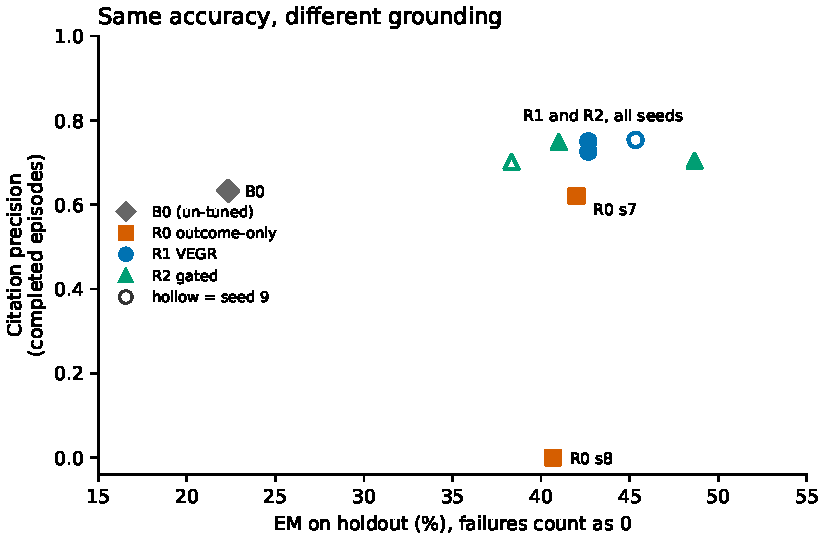
\includegraphics[keepaspectratio]{figures/fig4_3_em_vs_precision.pdf}}
\caption{Holdout EM (all episodes, failures counted as 0) against
citation precision (completed episodes), one point per
run.}\label{fig:4.3}
\end{figure}

\begin{itemize}
\tightlist
\item
  Shape and colour encode the reward. Hollow markers are seed-9 runs,
  whose values come from the run logs.
\item
  R1 and R2 cluster at precision 0.70--0.75. R0 seed 7 sits slightly
  lower, at 0.62. R0 seed 8 reaches the same EM with precision 0.
\end{itemize}

\textbf{Answer to RQ2 (so far).} VEGR matches the accuracy of
outcome-only reward and avoids its shortcuts on the seeds run so far.
The outcome-only reward can be satisfied without evidence, and which
shortcut the policy finds depends on the seed. The finding fits reward
hacking theory (Skalse et al., 2022): the outcome-only reward is a proxy
that does not include grounding, and on two of two seeds the policy
found a way to satisfy the proxy that the intended objective would
reject.

Two caveats limit how strong this claim is:

\begin{itemize}
\tightlist
\item
  R0 seed 9 will show whether a shortcut appears a third time.
  {[}TODO{]}
\item
  \textbf{Grounded EM} (EM = 1, at least one citation, every citation
  gold) will quantify the grounding gap in a single number. R0 seed 8's
  grounded EM is 0 by construction. Because R1's citation precision is
  only about 0.75, R1's grounded EM is also expected to be well below
  its EM. {[}TODO: grounded EM for all runs.{]}
\end{itemize}

\section{Diagnosis: why outcome-only reward is unstable}\label{sec:4.5}

\textbf{Zero-variance groups.} GRPO learns nothing from a group in which
all 8 rollouts receive the same reward (Section~\ref{sec:3.6}), and such
steps are skipped. Under the outcome-only reward this happens often,
because the reward is binary and many questions are either always solved
or never solved within a group.

\begin{longtable}[]{@{}ll@{}}
\caption{Skipped (zero-variance) training steps out of
256.}\label{tbl:4.3}\tabularnewline
\toprule\noalign{}
Run & Skipped steps \\
\midrule\noalign{}
\endfirsthead
\toprule\noalign{}
Run & Skipped steps \\
\midrule\noalign{}
\endhead
\bottomrule\noalign{}
\endlastfoot
R0 seed 7 & 107 \\
R0 seed 8 & 128 \\
R1 seed 7 & 8 \\
R1 seed 8 & 8 \\
R2 seed 7 & 19 \\
R2 seed 8 & 20 \\
Seed-9 runs & {[}TODO: metrics.jsonl not yet downloaded from the
pod{]} \\
\end{longtable}

R0 therefore learns from only about half of its questions, and each of
those gives only a coarse right-or-wrong signal. VEGR's continuous terms
(F1, coverage, precision, recall, penalties) almost always separate the
8 rollouts, so nearly every step produces a gradient.

Our interpretation, which these data support but do not prove, is that
with so few informative updates, whatever habit emerges early in R0
training gets reinforced and locked in. That would explain why the
failure mode differs between seeds. The R0-dyn run tests this directly
(Section~\ref{sec:4.6}).

\begin{figure}
\centering
\pandocbounded{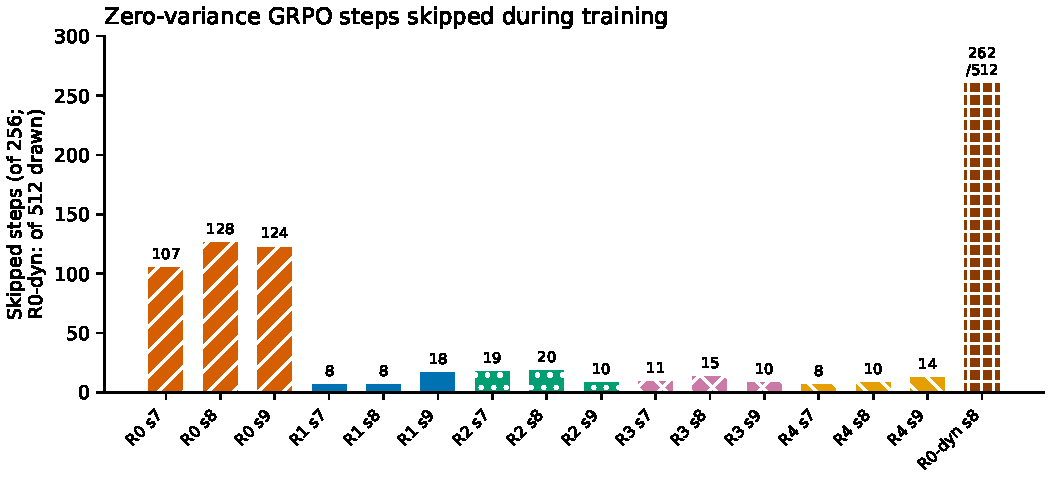
\includegraphics[keepaspectratio]{figures/fig4_1_skipped_steps.pdf}}
\caption{Number of GRPO training steps skipped because all 8 rollouts in
the group received the same reward, out of 256 steps per run.
Outcome-only runs (R0, hatched) skip 107--128 steps; VEGR (R1) skips 8
and gated VEGR (R2, dotted) skips 19--20. Source:
\texttt{metrics.\allowbreak{}jsonl} of each run; values in
\texttt{docs/\allowbreak{}thesis/\allowbreak{}figures/\allowbreak{}figures\_\allowbreak{}data.\allowbreak{}json}.}\label{fig:4.1}
\end{figure}

The training curve for seed 8 (Figure~\ref{fig:4.2}) shows when the R0
shortcut appeared. Over the first 64 steps, the two rewards produce
similar citation precision during training (R0 0.568 and 0.499; R1 0.550
and 0.520). R0 then falls to 0.126 in steps 65--96 and stays at 0.000
for every block from step 97 on, while R1 rises to between 0.62 and
0.76.

\begin{figure}
\centering
\pandocbounded{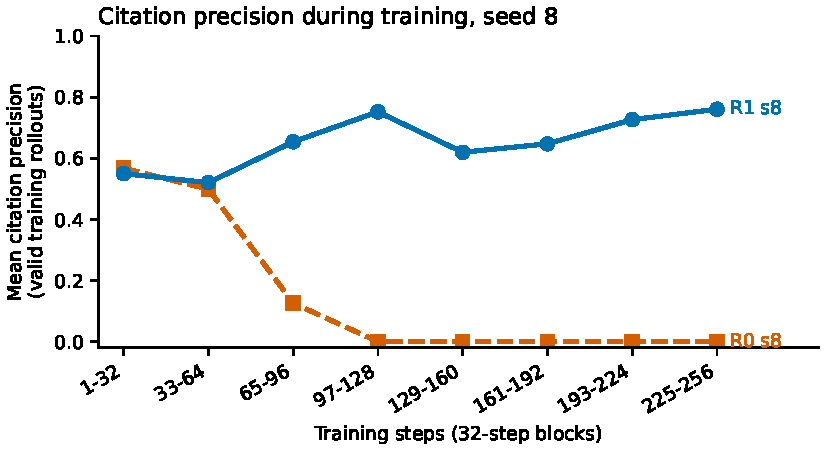
\includegraphics[keepaspectratio]{figures/fig4_2_citation_precision.pdf}}
\caption{Mean citation precision of valid training rollouts per 32-step
block, seed 8. A valid answer with no citations has precision 0 by
definition (Section~\ref{sec:3.4}). Each point averages 128--256 valid
rollouts. These are training rollouts sampled at temperature 1.0, not
holdout results. Source: \texttt{metrics.\allowbreak{}jsonl}; script
\texttt{scripts/\allowbreak{}make\_\allowbreak{}thesis\_\allowbreak{}figures.\allowbreak{}py}.}\label{fig:4.2}
\end{figure}

\textbf{``Precise but incomplete'' citations.} VEGR raises citation
precision (about 0.73--0.75, against 0.633 for B0) but not evidence
coverage, which ranges from 0.333 to 0.513 across R1 seeds. The citation
pattern of R1 seed 8 shows why:

\begin{itemize}
\tightlist
\item
  It cites 1 sentence in 97 episodes, 2 sentences in 182, and 3 in 8.
\item
  By sentence position, sentence 0 is cited 233 times, sentence 1 161
  times, and sentence 2 57 times.
\end{itemize}

\begin{figure}
\centering
\pandocbounded{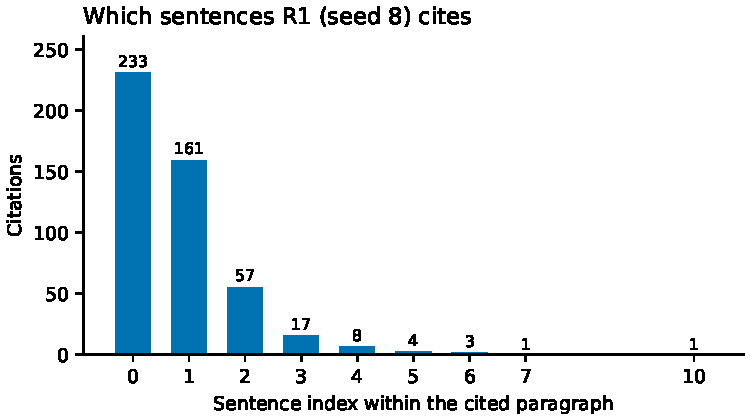
\includegraphics[keepaspectratio]{figures/fig4_7_cited_index.pdf}}
\caption{Position of every sentence cited by R1 seed 8 in its completed
holdout episodes (485 citations). 451 of them (93\%) point to one of the
first three sentences of a paragraph.}\label{fig:4.7}
\end{figure}

The policy prefers a few early sentences, which are usually correct but
often not the full gold evidence. HotpotQA's gold support often includes
sentences beyond index 0. Under a summed reward, citing one safe
sentence already earns full precision and partial coverage, so the
policy has little reason to risk adding more. This matches ALCE's
observation that citation precision and citation recall are distinct,
and that models tend to be precise but incomplete (Gao et al., 2023).

Coverage also varies between seeds. R1 seed 9 has the best EM (45.3\%)
but the lowest coverage (0.333). Coverage is therefore not a fixed
property of the reward, and higher accuracy does not imply more complete
citations.

\section{RQ3: Reward variants and optimizer fixes}\label{sec:4.6}

\textbf{R2 (gated penalties) is not better than R1.}

\begin{itemize}
\tightlist
\item
  On seed 8 alone, R2 looked like a clear win: 48.7\% against 42.7\%, a
  +6.0-point difference with 95\% CI {[}+1.3, +11.0{]}. This is the only
  reward-variant comparison whose CI excludes zero.
\item
  It \textbf{did not replicate}. On seed 7, R2 is 1.7 points below R1
  (CI {[}−7.0, +4.0{]}). On seed 9, R2 reaches 38.3\% against R1's
  45.3\%.
\item
  The 3-seed means are 42.7\% for R2 and 43.6\% for R1.
\item
  R2 also has the widest seed range of any method, from 38.3\% to 48.7\%
  (Figure~\ref{fig:4.4}).
\end{itemize}

\begin{figure}
\centering
\pandocbounded{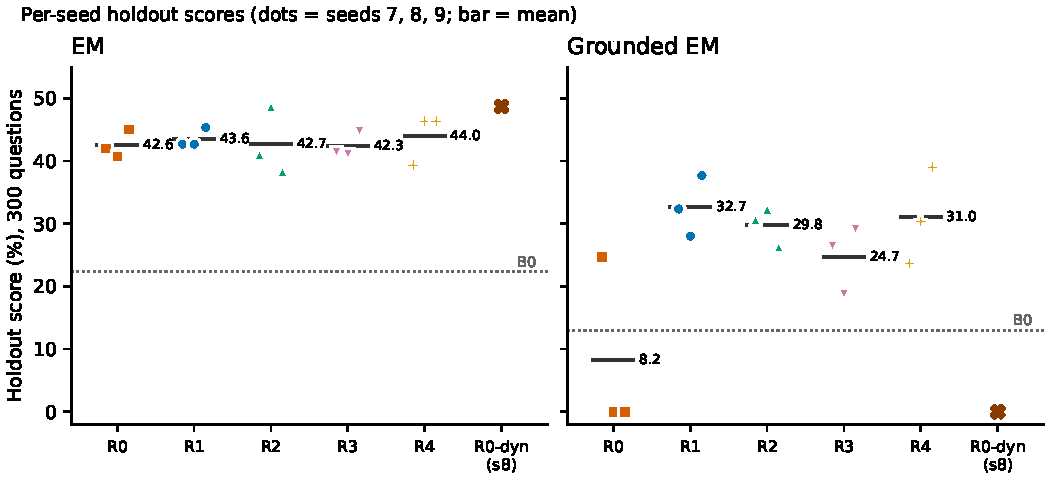
\includegraphics[keepaspectratio]{figures/fig4_4_em_per_seed.pdf}}
\caption{Holdout EM per seed for each reward. The horizontal bar is the
seed mean, and the dotted line is the un-tuned baseline B0
(22.3\%).}\label{fig:4.4}
\end{figure}

\begin{itemize}
\tightlist
\item
  R1's three seeds lie within about 3 points of each other, while R2's
  spread over 10.4 points.
\item
  Hollow markers (seed 9) are taken from the run logs on the training
  pod; their raw episode files are not yet downloaded.
\item
  R0 seed 9 is pending.
\end{itemize}

This is the kind of result Henderson et al.~(2018) and Agarwal et
al.~(2021) warn about: a single-seed comparison can look significant and
still not hold across seeds. Given seed ranges of up to about 10 EM
points, \textbf{this thesis does not claim method differences smaller
than about 6 points}. Every claimed difference must hold across seeds.

The following runs are exploratory follow-ups, designed after the
results above (Section~\ref{sec:3.8}):

\begin{itemize}
\tightlist
\item
  \textbf{R3 (coverage ×2):} does doubling the coverage weight raise
  evidence coverage, and at what cost in precision or EM? {[}TODO{]}
\item
  \textbf{R4 (VEGR + Dr.~GRPO):} does dropping the standard-deviation
  normalization change stability across seeds? {[}TODO{]}
\item
  \textbf{R0-dyn (R0 + dynamic sampling, seed 8):} this is the key
  control. If dynamic sampling alone prevents the seed-8 citation
  shortcut, the instability comes from the optimizer, not the reward. If
  the shortcut still appears, the evidence terms in the reward are
  needed. {[}TODO{]}
\end{itemize}

\section{Error analysis and example traces}\label{sec:4.7}

\textbf{Failure categories.} Table~\ref{tbl:4.4} lists the episodes that
did not complete.

\begin{longtable}[]{@{}lllll@{}}
\caption{Failed episodes out of 300, by type (evidence / protocol /
budget).}\label{tbl:4.4}\tabularnewline
\toprule\noalign{}
Run & Evidence & Protocol & Budget & Total \\
\midrule\noalign{}
\endfirsthead
\toprule\noalign{}
Run & Evidence & Protocol & Budget & Total \\
\midrule\noalign{}
\endhead
\bottomrule\noalign{}
\endlastfoot
B0 & 85 & 37 & 8 & 130 \\
R0 s7 & 14 & 7 & 1 & 22 \\
R0 s8 & 0 & 1 & 0 & 1 \\
R1 s7 & 8 & 5 & 0 & 13 \\
R1 s8 & 8 & 5 & 0 & 13 \\
R1 s9 & -- & -- & -- & 7 \\
R2 s7 & 10 & 7 & 0 & 17 \\
R2 s8 & 3 & 7 & 0 & 10 \\
R2 s9 & -- & -- & -- & 14 \\
\end{longtable}

{[}TODO: per-type breakdown for seed 9.{]}

\begin{figure}
\centering
\pandocbounded{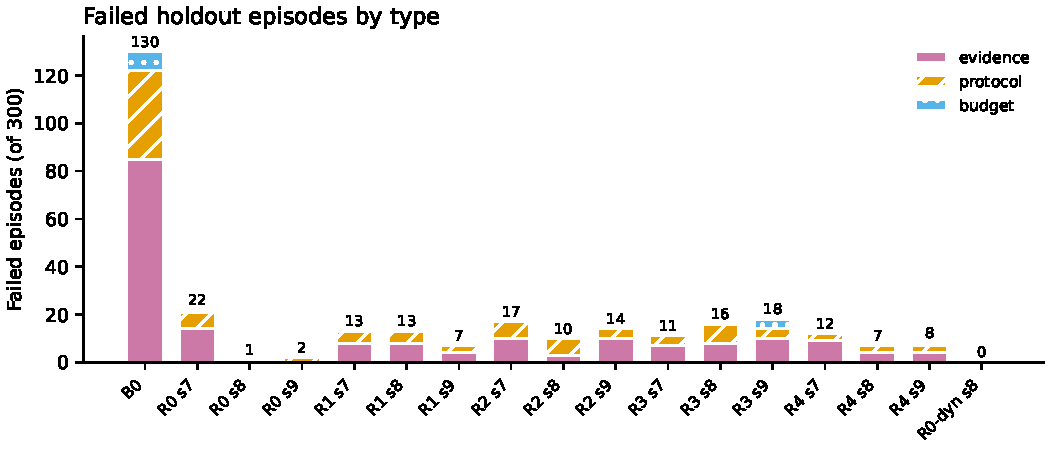
\includegraphics[keepaspectratio]{figures/fig4_6_failures.pdf}}
\caption{Failed holdout episodes per run, stacked by failure type
(seed-7 and seed-8 runs; seed-9 breakdown pending). Training removes
most failures of every type. Evidence failures (invented or
unretrievable citations) shrink from 85 to between 3 and 14 in the runs
where the agent still cites.}\label{fig:4.6}
\end{figure}

R0 seed 8 has almost no failures, but for a degenerate reason. An answer
without citations can never produce an evidence failure, so the citation
shortcut removes that failure type entirely.

\textbf{Example traces.} The traces below are taken verbatim from the
holdout episode logs of the seed-7 and seed-8 runs.

\emph{Trace 1: same question, three behaviours} (question
\texttt{5adbf0a255429947ff17385a}). All three policies answer correctly
(EM = 1).

\begin{Verbatim}
R1 s8:  SEARCH[Laleli Mosque Esma Sultan Mansion location]
        SEARCH[Laleli neighborhood]
        ANSWER[no] CITATIONS[Laleli Mosque|0; Esma Sultan Mansion|0]
R0 s8:  SEARCH[Laleli Mosque and Esma Sultan Mansion location]
        ANSWER[no]
R0 s7:  SEARCH[neighborhood of Laleli Mosque and Esma Sultan Mansion]
        SEARCH[neighborhood of Laleli Mosque and Esma Sultan Mansion]
        SEARCH[neighborhood of Laleli Mosque and Esma Sultan Mansion]
        ANSWER[no] CITATIONS[Esma Sultan Mansion|0; Laleli Mosque|0]
\end{Verbatim}

\begin{itemize}
\tightlist
\item
  \textbf{R1 (VEGR)} searches twice with different queries and cites one
  sentence from each gold paragraph. In this episode coverage and
  precision are both 1.0.
\item
  \textbf{R0 seed 8} answers after one search with no citations: the
  citation shortcut.
\item
  \textbf{R0 seed 7} repeats the same query three times before
  answering: duplicate-search spam.
\end{itemize}

\emph{Trace 2: citation shortcut on a different question}
(\texttt{5abd94525542992ac4f382d2}).

\begin{Verbatim}
R1 s8:  SEARCH[S/S 2014 debut South Korean boy group]
        SEARCH[WINNER YG Entertainment]
        ANSWER[YG Entertainment] CITATIONS[2014 S/S|0; Winner (band)|0]
R0 s8:  SEARCH[2014 S/S debut album South Korean boy group formed by]
        ANSWER[YG Entertainment]
\end{Verbatim}

R1 uses its second search to follow the bridge entity (``WINNER'') into
the second paragraph, which is the multi-hop behaviour the task is meant
to require. R0 seed 8 gives the same answer with nothing to support it.

\emph{Trace 3: an evidence failure (R1 s8).} The final action
\texttt{ANSWER{[}yes{]} CITATIONS{[}Ambroise Thomas|0; Provesi|1{]}}
(question \texttt{5ab29c24554299449642c932}) was marked invalid as an
evidence failure: ``citation references unknown document `Provesi'\,''.
The model cited a document title that had not appeared in any of its
search results. Even after training, invented or unretrievable citations
remain the most common failure type for R1 and R2 (Table~\ref{tbl:4.4}).

{[}TODO: add 2--5 more traces, including a protocol failure and an R3
trace, once the fixes batch is in.{]}

\section{Discussion}\label{sec:4.8}

\textbf{Comparison with the literature.}

\begin{itemize}
\tightlist
\item
  \textbf{Shortcut behaviour.} The R0 shortcuts are consistent with CaRR
  (Zhang et al., 2026), which reports that outcome-only GRPO agents
  learn shortcut answers and use fewer tool calls. R0 seed 8 shows the
  same pattern in a much smaller setting (7B, LoRA, 256 questions, one
  GPU). Because HotpotQA's supporting facts are exact, the shortcut can
  be detected by rule, without a judge.
\item
  \textbf{Seed dependence.} R0 seed 7 failed in the \emph{opposite}
  direction from seed 8: it searched more, not less. So ``fewer
  searches'' is not the only way outcome-only training goes wrong.
\item
  \textbf{Accuracy.} The results agree with Search-R1 (Jin et al., 2025)
  that outcome-only RL improves accuracy. They add that the accuracy
  number alone hides whether the answers are grounded.
\end{itemize}

\textbf{What the results support:}

\begin{enumerate}
\def\labelenumi{\arabic{enumi}.}
\tightlist
\item
  GRPO with LoRA on one GPU improves a 7B search agent by roughly 18--26
  EM points over the un-tuned model. Most of the gain comes from
  learning to produce valid, verifiable actions.
\item
  Outcome-only and evidence-grounded rewards reach statistically
  indistinguishable accuracy.
\item
  The outcome-only reward produced a different shortcut on each of two
  seeds, while VEGR stayed consistent in grounding across three seeds.
\end{enumerate}

\textbf{What the results do not support:}

\begin{itemize}
\tightlist
\item
  That VEGR is more \emph{accurate} than outcome-only reward.
\item
  That gated penalties (R2) help.
\item
  That VEGR solves evidence coverage. It does not; coverage remains the
  main open problem.
\end{itemize}

\textbf{Threats to validity.}

\begin{itemize}
\tightlist
\item
  \textbf{Few seeds, small holdout.} Three seeds and 300 holdout
  questions cannot resolve differences smaller than about 6 EM points.
  R0 currently has only two seeds.
\item
  \textbf{Closed corpus.} Retrieval is BM25 over each question's own 10
  paragraphs, not an open corpus or the web. The search problem is much
  easier than in deployed agents.
\item
  \textbf{Small training scale.} Each run uses 256 questions for one
  epoch with a LoRA-adapted 7B model. The results may not hold at larger
  scale.
\item
  \textbf{Software change.} The PyTorch version changed between B0/R1
  seed 7 (2.14.1) and the later runs (2.11.0) because of a driver
  constraint.
\item
  \textbf{Environment loophole.} The environment accepts answers without
  citations. This was kept deliberately for comparability, but it makes
  the R0 seed-8 shortcut possible. Closing it would likely change R0's
  behaviour.
\item
  \textbf{Untuned weights.} The reward weights are untuned defaults.
\item
  \textbf{Exploratory runs.} R3, R4 and R0-dyn were designed after
  seeing the R0/R1/R2 results and are reported as exploratory.
\item
  \textbf{R0-dyn has one seed.} Budget allowed only a single run, on the
  seed where R0 collapsed (Section~\ref{sec:3.8}). Its result is
  evidence about mechanism on that seed, not a method comparison.
\end{itemize}

\chapter{Conclusion}\label{sec:5}

\begin{quote}
\textbf{DRAFT --- not submission-ready.} Every number below is taken
from Chapter~\ref{sec:4} and has the same sources.
\end{quote}

\section{Summary}\label{sec:5.1}

This thesis asked whether a search agent trained with reinforcement
learning can be rewarded for \emph{grounded} answers, rather than only
correct ones, without an LLM judge and on a student budget. A
Qwen2.5-7B-Instruct agent with LoRA was trained with GRPO on HotpotQA.
It searched each question's paragraphs with BM25 and answered with
sentence-level citations, which a rule could check against HotpotQA's
gold supporting facts. Sixteen runs were trained on one GPU for about
\$49 in total: five reward and optimizer configurations on three seeds
each, plus one diagnostic run. Each was evaluated on a frozen
300-question holdout.

\textbf{RQ1: Does GRPO training improve a 7B search agent over the
un-tuned model?} Yes. Every method gains about +20 EM points over the
un-tuned model (22.3\%), and every confidence interval excludes zero.
Most of the gain comes from learning the action protocol: the un-tuned
model fails 130 of 300 episodes, while trained runs fail at most 22.

\textbf{RQ2: Does VEGR prevent the shortcuts of answer-only reward
without losing accuracy?} Yes. The two rewards reach the same accuracy
(43.6\% vs.~42.6\%, a difference of +1.0 points with CI {[}−1.9,
+3.8{]}). VEGR's grounded EM is \textbf{24.4 points higher} (CI
{[}+20.9, +28.1{]}). All three outcome-only seeds ended in a degenerate
behaviour. Two stopped citing entirely, and the third repeated the same
search in most episodes. As a result, the outcome-only agent is
\emph{less} grounded than the un-tuned model (−4.8 grounded EM points).
VEGR kept citation precision at 0.73--0.75 on every seed.

\textbf{RQ3: How do reward variants and optimizer fixes affect grounding
and search behaviour?} None improved on plain VEGR.

\begin{itemize}
\tightlist
\item
  Gated penalties (R2) and Dr.~GRPO advantages (R4) made no measurable
  difference. R2's apparent single-seed gain of +6 EM points did not
  replicate.
\item
  Doubling the coverage weight (R3) raised evidence coverage from 0.44
  to 0.57. Precision fell, and grounded EM dropped 8.0 points.
\item
  Dynamic sampling (R0-dyn, one seed) made the outcome-only agent more
  accurate (+8.0 EM points). It still cited nothing and collapsed during
  training on the same schedule as the plain outcome-only run.
\end{itemize}

The citation shortcut is therefore caused by what the reward asks for,
not only by how GRPO uses it.

\section{Contributions}\label{sec:5.2}

\begin{enumerate}
\def\labelenumi{\arabic{enumi}.}
\tightlist
\item
  \textbf{VEGR}, a judge-free, sentence-level evidence reward that also
  enforces the action protocol. Its individual terms are not new; the
  contribution is the combination and its controlled evaluation.
\item
  \textbf{Evidence that answer-only GRPO produces shortcuts} in a small,
  reproducible setting, detectable by rule. The thesis also diagnoses
  the shortcut: outcome-only runs skip about half their training steps
  for lack of reward variance, but restoring those updates does not
  prevent the shortcut.
\item
  \textbf{A controlled multi-seed comparison} with paired bootstrap
  confidence intervals and seed standard deviations. It separates reward
  design from optimizer fixes, and shows how a single-seed result can
  mislead.
\item
  \textbf{An open single-GPU pipeline.} One run costs about \$2.25.
  Splits, configurations, logs, per-episode results and the figure
  script are released in the repository.
\end{enumerate}

\section{Limitations}\label{sec:5.3}

\begin{itemize}
\tightlist
\item
  \textbf{Setting.} Retrieval is BM25 over each question's own 10
  paragraphs, on one dataset, so the search problem is far easier than
  open-web search.
\item
  \textbf{Scale.} Training uses 256 questions per run for one epoch, on
  a 7B model with LoRA.
\item
  \textbf{Statistics.} Three seeds and 300 holdout questions resolve
  large effects, such as the grounded-EM gaps. They cannot resolve EM
  differences of a few points.
\item
  \textbf{Single seed for R0-dyn.} R0-dyn has one seed and reached 250
  of its 256 target updates.
\item
  \textbf{Exploratory runs.} R3, R4 and R0-dyn were designed after
  seeing the first results.
\item
  \textbf{Loophole and weights.} The environment accepts uncited
  answers. The reward weights were not tuned.
\item
  \textbf{Coverage.} Coverage remains low. Even with VEGR, about a
  quarter of correct answers include at least one non-gold citation.
\end{itemize}

\section{Future work}\label{sec:5.4}

\begin{itemize}
\tightlist
\item
  \textbf{Close the no-citation loophole and fix the citation format.}
  Require at least one citation, and use a separator that cannot occur
  in titles (Trace 5, Section~\ref{sec:4.7}). Then test whether
  outcome-only training finds a different shortcut.
\item
  \textbf{Reward complete evidence without losing precision.} Examples
  are a coverage term that counts only gold citations, or a reward based
  on the F1 of the citation set, instead of a larger weight on coverage
  alone (R3).
\item
  \textbf{Step-level credit.} Reward individual searches by the
  information they add, in the direction of STAMP (Xu et al., 2026),
  rather than scoring only the final episode.
\item
  \textbf{Harder retrieval and more data.} Extend to an open corpus, to
  other multi-hop datasets with gold evidence such as 2WikiMultiHopQA
  and MuSiQue, and to larger training sets.
\item
  \textbf{More seeds for the diagnostic runs.} Run R0-dyn on all three
  seeds, so that the mechanism finding becomes a method comparison.
\end{itemize}


\appendix
\chapter{Full Agent Prompt}\label{sec:A}

This appendix gives the complete prompt the agent receives, for one real
holdout question. The text was produced by
\texttt{build\_\allowbreak{}prompt}
(\texttt{src/\allowbreak{}needle/\allowbreak{}inference/\allowbreak{}runner.\allowbreak{}py}),
the same function used in training and evaluation. It is passed to
Qwen2.5-7B-Instruct as a single user message through the model's chat
template.

\section{How the example was
reproduced}\label{how-the-example-was-reproduced}

\begin{itemize}
\tightlist
\item
  \textbf{Question:} \texttt{5abd94525542992ac4f382d2} from the frozen
  holdout
  (\texttt{configs/\allowbreak{}evaluation/\allowbreak{}holdout\_\allowbreak{}v1\_\allowbreak{}ids.\allowbreak{}json}).
  The row was taken from the HotpotQA distractor validation split on
  Hugging Face (\texttt{hotpotqa/\allowbreak{}hotpot\_\allowbreak{}qa},
  \texttt{distractor/\allowbreak{}validation-\allowbreak{}00000-\allowbreak{}of-\allowbreak{}00001.\allowbreak{}parquet})
  and converted to the native HotpotQA format.
\item
  \textbf{History:} a \texttt{SearchEnvironment} (top-k = 3, budget = 3)
  replayed the two searches that R1 seed 8 made in its holdout episode
  (\texttt{results/\allowbreak{}2026-\allowbreak{}10-\allowbreak{}10-\allowbreak{}batch/\allowbreak{}r1\_\allowbreak{}full\_\allowbreak{}seed8/\allowbreak{}episodes.\allowbreak{}jsonl}).
  \texttt{build\_\allowbreak{}prompt} was then called at the point where
  the agent chose its final action.
\item
  \textbf{Gold supporting facts:} \texttt{2014 S/\allowbreak{}S|0} and
  \texttt{Winner (band)|0}.
\item
  \textbf{Agent's action at this point:}
  \texttt{ANSWER{[}YG Entertainment{]} CITATIONS{[}2014 S/\allowbreak{}S|0; Winner (band)|0{]}}.
  The answer is correct and both gold sentences are cited
  (Table~\ref{tbl:3.1}, episode A).
\end{itemize}

\section{Prompt text}\label{prompt-text}

The prompt is reproduced verbatim. The leading spaces on some sentences
are present in the HotpotQA source text.

\begin{Verbatim}
You are a careful evidence-seeking QA agent.
Return exactly one action: SEARCH[query] or ANSWER[answer] CITATIONS[title|index; ...].
SEARCH[query] is search-only: never append CITATIONS[...] to a SEARCH action.
ANSWER[...] is terminal; when the search budget reaches 0, answer immediately.
Example: ANSWER[United States] CITATIONS[Ursula K. Le Guin|1; The Left Hand of Darkness|1].
Use one title|index citation per entry; separate entries with semicolons, never comma-separated indices.
Do not add a period, explanation, or any text after the final closing bracket.
Copy citation titles exactly as shown in the search results, including punctuation and accents.
Never invent a document title; use CITATIONS[] when no citation can be validated.
Use only the supplied search results for citations.
Question: 2014 S/S is the debut album of a South Korean boy group that was formed by who?
Remaining search budget: 1
Search results so far:
Search 1: S/S 2014 debut South Korean boy group
[2014 S/S]
0: 2014 S/S is the debut album of South Korean group WINNER.
1:  It was released on August 12, 2014 by the group's record label, YG Entertainment.
2:  The members were credited for writing the lyrics and composing the majority of the album's songs.
[History (band)]
0: History (Korean: [Hangul] ) was a South Korean boy group formed by LOEN Entertainment in 2013.
1:  They debuted on April 26, 2013 with "Dreamer", featuring the narration of their labelmate IU.
2:  They were LOEN Entertainment's first boy group.
3:  They officially disbanded on May 12, 2017.
[SF9 (band)]
0: SF9 (Korean: [Hangul] ; shortened from Sensational Feeling 9) is a South Korean boy group formed by FNC Entertainment.
1:  SF9 is the company's first dance boy group to ever debut.
2:  SF9 debuted on October 5, 2016 with the release of their first single album "Feeling Sensation".
Search 2: WINNER YG Entertainment
[Winner (band)]
0: Winner (Hangul: [Hangul]), often stylized as WINNER, is a South Korean boy group formed in 2013 by YG Entertainment and debuted in 2014.
1:  It currently consists of four members, Jinwoo, Seunghoon, Mino and Seungyoon.
2:  Originally a five-piece group with Taehyun, who later departed from the group in November 2016.
[2014 S/S]
0: 2014 S/S is the debut album of South Korean group WINNER.
1:  It was released on August 12, 2014 by the group's record label, YG Entertainment.
2:  The members were credited for writing the lyrics and composing the majority of the album's songs.
[History (band)]
0: History (Korean: [Hangul] ) was a South Korean boy group formed by LOEN Entertainment in 2013.
1:  They debuted on April 26, 2013 with "Dreamer", featuring the narration of their labelmate IU.
2:  They were LOEN Entertainment's first boy group.
3:  They officially disbanded on May 12, 2017.
\end{Verbatim}

\section{Notes on the prompt}\label{notes-on-the-prompt}

\begin{itemize}
\tightlist
\item
  \textbf{First turn.} Before any search, the history section reads
  \texttt{(none)} and the remaining budget is 3.
\item
  \textbf{Repeated documents.} Each search lists its full top-3 results,
  even when a document was already returned by an earlier search (``2014
  S/S'' and ``History (band)'' appear twice above). The prompt grows
  with every search, which is one reason the budget is limited to 3.
\item
  \textbf{Why the format rules exist.} The rules about citation
  formatting (one \texttt{title|index} per entry, exact titles, no
  trailing text) target the protocol failures observed in the un-tuned
  model, which lost 37 of 300 holdout episodes to malformed actions
  (Section~\ref{sec:4.2}).
\item
  \textbf{No-citation loophole.} The line ``use CITATIONS{[}{]} when no
  citation can be validated'' is what makes an empty citation list a
  valid action (the loophole discussed in Section~\ref{sec:3.3}).
\end{itemize}


\end{document}
